\documentclass[12pt,a4paper]{article}

% Packages
\usepackage[utf8]{inputenc}
\usepackage[english]{babel}
\usepackage{geometry}
\usepackage{graphicx}
\usepackage{amsmath}
\usepackage{amssymb}
\usepackage{booktabs}
\usepackage{caption}
\usepackage{subcaption}
\usepackage{hyperref}
\usepackage{cite}
\usepackage{natbib}
\usepackage{url}
\usepackage{float}
\usepackage{enumitem}
\usepackage{setspace}
\usepackage{fancyhdr}
\usepackage{tikz}
\usepackage{pgfplots}
\pgfplotsset{compat=1.18}
\usepackage{multirow}
\usepackage{longtable}
\usepackage{array}
\usepackage{appendix}
\usepackage{listings}
\usepackage{xcolor}
\usepackage{multicol}

% Page geometry
\geometry{
    left=1in,
    right=1in,
    top=1in,
    bottom=1in
}

% Hyperref setup
\hypersetup{
    colorlinks=true,
    linkcolor=blue,
    filecolor=magenta,      
    urlcolor=cyan,
    citecolor=blue,
    pdftitle={ESG News Sentiment and Market Risk},
    pdfauthor={Anindita, Ogunlowo},
}

% Header and footer
\pagestyle{fancy}
\fancyhf{}
\fancyhead[L]{ESG News Sentiment and Market Risk}
\fancyhead[R]{\thepage}
\renewcommand{\headrulewidth}{0.4pt}

% Code listing style
\lstset{
    language=Python,
    basicstyle=\ttfamily\small,
    keywordstyle=\color{blue},
    commentstyle=\color{gray},
    stringstyle=\color{red},
    showstringspaces=false,
    breaklines=true,
    frame=single,
    numbers=left,
    numberstyle=\tiny\color{gray}
}

% Custom commands
\newcommand{\code}[1]{\texttt{#1}}
\newcommand{\figref}[1]{Figure~\ref{#1}}
\newcommand{\tabref}[1]{Table~\ref{#1}}
\newcommand{\eqref}[1]{Equation~\ref{#1}}
\newcommand{\secref}[1]{Section~\ref{#1}}

% Title information
\title{
    \vspace{-2cm}
    \textbf{\LARGE ESG News Sentiment and Market Risk:} \\
    \vspace{0.3cm}
    \textbf{\LARGE Evidence from Global News Data} \\
    \vspace{1cm}
    \normalsize Final Project Report \\
    \normalsize Sustainable Investment (FRE GY 6951)
}

\author{
    Azfina Putri Anindita\thanks{apa9951@nyu.edu} \quad
    Muhideen (Damola) Ogunlowo\thanks{mao9295@nyu.edu}
    \\
    \normalsize New York University \\
    \normalsize Tandon School of Engineering \\
    \normalsize Department of Finance and Risk Engineering \\
    \vspace{0.5cm}
    \normalsize Supervised by Prof. Bruno G. Kamdem, Ph.D.
}

\date{\today}

\begin{document}

% Title page
\maketitle
\thispagestyle{empty}

\vfill

\begin{abstract}
\noindent
Environmental, social, and governance (ESG) risks have become increasingly important for financial markets as sustainability-related issues continue to intensify. This study constructs an ESG Sentiment Index from global news data and examines its relationship with short-term market risk, measured through returns and volatility. Using data from the GDELT Project and Yahoo Finance for the period April 3, 2014 to February 19, 2015, we analyze whether ESG-related news sentiment is correlated with market behavior and whether it can serve as an early warning indicator for sustainable investment risk management. Our findings suggest that ESG news sentiment exhibits a statistically significant negative relationship with short-term market volatility ($r = -0.136$, $p < 0.05$), while its association with daily returns is positive but weak and statistically insignificant. Lagged ESG sentiment variables show stronger predictive power for volatility up to five trading days ahead, with the three-day lag yielding the highest correlation ($r = -0.293$, $p < 0.05$). Lasso feature selection identifies rolling average sentiment and lagged sentiment (lags 2, 3, and 5) as the most relevant predictors of future volatility, providing evidence that ESG news data adds incremental explanatory power beyond traditional financial indicators. These results have important implications for investors, risk managers, and regulators seeking to integrate ESG considerations into financial risk assessment frameworks.
\end{abstract}

\noindent
\textbf{Keywords:} ESG, Sentiment Analysis, Market Risk, Volatility, News Data, Sustainable Investment, Financial Stability

\vfill

\clearpage

% Table of Contents
\tableofcontents
\clearpage

% List of Figures
\listoffigures
\clearpage

% List of Tables
\listoftables
\clearpage

%----------------------------------------------------------------------------------------
% MAIN CONTENT
%----------------------------------------------------------------------------------------

\onehalfspacing

\section{Introduction}
\label{sec:introduction}

\subsection{Background and Motivation}
\label{subsec:background}

Environmental, social, and governance (ESG) risks have emerged as critical factors in financial markets, driven by intensifying sustainability-related challenges such as climate change, social inequality, and governance failures \citep{friede2015esg}. These risks often materialize through news events—including extreme weather incidents, environmental accidents, corporate governance scandals, and social controversies—that can affect investor sentiment and market expectations before their financial impacts are fully reflected in asset prices.

Despite the growing importance of ESG considerations, traditional financial risk models continue to rely heavily on historical market data such as prices, returns, and volatility \citep{baker2016measuring}. These models may not fully capture emerging sustainability-related risks, particularly those that develop gradually or originate outside the financial system. As a result, investors and regulators may underestimate ESG-related risks until they become financially material, potentially increasing exposure to sudden market adjustments and instability.

At the same time, the availability of large-scale news data has created new opportunities to quantify qualitative information such as sentiment and public attention. Global news databases like the GDELT Project make it possible to systematically track how environmental, social, and governance topics are reported across countries and over time \citep{leetaru2013gdelt}. Previous research demonstrates that news-based sentiment indicators can influence market behavior and are useful for understanding uncertainty and risk in financial markets \citep{tetlock2007giving}.

\subsection{Research Gap}
\label{subsec:gap}

However, the application of news sentiment specifically to ESG risk monitoring remains relatively underexplored in the context of sustainable investment. While studies have examined the relationship between ESG ratings and financial performance \citep{amel2018esg}, the potential of real-time news sentiment as an early warning signal for ESG-related market risk has received limited attention.

To further ground the motivation of this study, we note recent real-world examples where ESG-related risks surfaced rapidly through news coverage before being fully reflected in market prices. For instance, during 2024–2025, global sustainable funds experienced record net outflows—reversing previous inflows and reflecting a shift in investor sentiment around ESG strategies that was widely covered by financial media. These episodes illustrate how sustainability-related risks may materialize first through heightened media attention and public concern, rather than immediately through observable market data.

\subsection{Research Objectives}
\label{subsec:objectives}

This study addresses the identified gap by constructing an ESG Sentiment Index using global news data and examining its relationship with short-term market risk. Specifically, we aim to:

\begin{enumerate}[itemsep=0.5em]
    \item Construct an ESG-related news sentiment index using global news data from the GDELT Project;
    \item Examine the relationship between ESG news sentiment and market risk (returns and volatility);
    \item Assess whether ESG news sentiment provides additional information beyond traditional financial indicators for market risk monitoring.
\end{enumerate}

These three objectives correspond to the following research questions addressed throughout the study:
\begin{enumerate}[itemsep=0.3em, label=\textbf{RQ\arabic*.}]
    \item Is ESG-related news sentiment correlated with market returns and volatility?
    \item Do negative ESG news signals increase short-term market risk, especially within 5 working days?
    \item Can ESG news sentiment serve as an early warning indicator (within 5 working days) for sustainable investment risk management?
\end{enumerate}

\subsection{Contribution and Relevance}
\label{subsec:contribution}

This project contributes to sustainable investment and sustainability management by connecting ESG information, data analytics, and financial risk assessment in a practical and data-driven manner. The focus on an index-based approach allows ESG-related information to be summarized into a single, interpretable metric that can be tracked over time. From a sustainable investment perspective, such an index may help investors incorporate ESG risks into risk assessment and portfolio monitoring. From a regulatory and policy perspective, including that of central banks, ESG sentiment indicators may support early warning systems for financial stability by highlighting periods of elevated sustainability-related risk \citep{ngfs2019call}.

\subsection{Report Structure}
\label{subsec:structure}

The remainder of this report is organized as follows: \secref{sec:literature} reviews relevant literature on ESG and financial markets, news sentiment analysis, and market risk. \secref{sec:methodology} describes the data sources, ESG keyword classification, sentiment aggregation methodology, and statistical models employed. \secref{sec:data} presents descriptive statistics and exploratory data analysis. \secref{sec:results} reports the main empirical findings. \secref{sec:discussion} discusses the implications, limitations, and potential applications. Finally, \secref{sec:conclusion} concludes and suggests directions for future research.

%----------------------------------------------------------------------------------------

\section{Literature Review}
\label{sec:literature}

\subsection{ESG and Financial Performance}
\label{subsec:lit-esg}

The relationship between ESG factors and financial performance has been extensively studied in recent decades. \citet{friede2015esg} conducted a meta-analysis of over 2,000 empirical studies and found that the majority show a non-negative relationship between ESG and corporate financial performance. However, the mechanisms through which ESG factors affect financial outcomes remain an active area of research.

More recently, attention has shifted from static ESG ratings to dynamic ESG information flows. \citet{amel2018esg} surveyed investment professionals and found that investors increasingly use ESG information not just for screening but for active risk management and alpha generation.

\subsection{News Sentiment and Market Behavior}
\label{subsec:lit-sentiment}

A growing body of literature examines how news sentiment affects financial markets. \citet{tetlock2007giving} demonstrated that negative media content predicts downward pressure on market prices, with effects persisting for several trading days. \citet{baker2016measuring} developed the Economic Policy Uncertainty (EPU) index based on newspaper coverage, showing that policy-related uncertainty significantly impacts investment, employment, and stock market volatility.

These studies suggest that news-based measures can capture market-relevant information that may not be immediately reflected in traditional financial indicators.

\subsection{ESG News and Market Risk}
\label{subsec:lit-esg-risk}

The specific intersection of ESG news sentiment and market risk is less explored. Some recent studies have begun to investigate this relationship. For example, research on climate-related news has shown that extreme weather events and climate policy announcements can trigger market reactions, particularly in carbon-intensive sectors.

\subsection{Early Warning Indicators}
\label{subsec:lit-early-warning}

The concept of early warning indicators is well-established in financial stability monitoring. Central banks and regulators use various leading indicators to anticipate financial stress \citep{ngfs2019call}. However, the integration of ESG-specific sentiment indicators into these frameworks is still nascent.

This study builds on these strands of literature by developing a comprehensive ESG news sentiment index and testing its predictive power for short-term market risk, with particular attention to the temporal dynamics of the relationship.

%----------------------------------------------------------------------------------------

\section{Methodology}
\label{sec:methodology}

\subsection{Conceptual Framework}
\label{subsec:framework}

Our analysis is guided by the following conceptual framework: ESG-related news events generate public attention and sentiment, which may affect investor expectations and risk perceptions. These sentiment shifts may precede or coincide with changes in market behavior, manifested as changes in returns and volatility. We hypothesize that negative ESG news sentiment is associated with higher market risk (lower returns and/or higher volatility), and that this relationship may have a temporal structure, with sentiment acting as a leading indicator.


\subsection{Data Sources}
\label{subsec:data-sources}

\subsubsection{ESG News Data: GDELT Project}
\label{subsubsec:gdelt}

We obtain ESG-related news data from the GDELT Project \citep{leetaru2013gdelt}, a global database of news events updated every 15 minutes. GDELT processes news articles from thousands of sources worldwide and provides pre-computed sentiment scores (Tone) ranging from -100 (extremely negative) to +100 (extremely positive).

We access GDELT data through Google BigQuery using the \code{gdelt-bq.gdeltv2.gkg\_partitioned} dataset. News articles are filtered based on predefined ESG keywords (described in \secref{subsec:keywords}).

\textbf{Data period:} April 3, 2014 -- February 19, 2015 \\
\textbf{Total articles collected:} 2,020 (912 ESG-tagged; 45.1\%)

\subsubsection{Market Data: Yahoo Finance}
\label{subsubsec:yfinance}

Market data are obtained from Yahoo Finance via the \code{yfinance} Python library. Consistent with the proposed methodology, we use \code{yfinance} for four purposes:

\begin{enumerate}[itemsep=0.3em]
    \item \textbf{Returns and volatility:} Daily adjusted closing prices for the S\&P 500 Index (\^{}GSPC); daily returns and rolling standard deviation of returns to compute 5-day and 20-day annualized volatility.
    \item \textbf{Traditional financial variables:} Fundamental indicators including market capitalization, price-to-earnings ratio, book-to-market ratio, leverage, and profitability ratios (ROE, ROA).
    \item \textbf{Market risk variables:} Market index data for the S\&P 500 to compute systematic risk measures.
    \item \textbf{Control variables:} Firm size, trading volume, and dividend yields for use in regression analysis.
\end{enumerate}

From the price data, we calculate:
\begin{itemize}[itemsep=0.3em]
    \item Daily returns: $R_t = \frac{P_t - P_{t-1}}{P_{t-1}}$
    \item Rolling volatility (5-day and 20-day): $\sigma_t = \text{std}(R_{t-k:t}) \times \sqrt{252}$
\end{itemize}

\subsection{ESG Keyword Classification}
\label{subsec:keywords}

To identify ESG-related news, we develop a structured set of keywords aligned with environmental, social, and governance dimensions. The keyword selection is based on ESG frameworks used by rating agencies and sustainability reporting standards (e.g., GRI, SASB).

\subsubsection{Environmental Keywords (E)}
\begin{itemize}[itemsep=0.2em]
    \item Climate: carbon emissions, climate change, climate transition, global warming, greenhouse gas
    \item Pollution: environmental spill, oil spill, toxic waste, water pollution
    \item Resource use: renewable energy, deforestation, water scarcity
    \item Compliance: environmental disaster, environmental compliance, carbon footprint
\end{itemize}

\subsubsection{Social Keywords (S)}
\begin{itemize}[itemsep=0.2em]
    \item Labor: labor strike, worker protest, workplace safety, employee welfare
    \item Human rights: human rights, labor rights, child labor, forced labor
    \item Diversity: diversity, inclusion, discrimination, gender equality
    \item Community: community impact, social responsibility, consumer safety
\end{itemize}

\subsubsection{Governance Keywords (G)}
\begin{itemize}[itemsep=0.2em]
    \item Board: board diversity, board independence, corporate governance
    \item Ethics: corporate fraud, accounting scandal, insider trading, corruption, bribery
    \item Transparency: disclosure, reporting standards, audit quality
    \item Compliance: regulatory violation, ethics violation, regulatory fine
\end{itemize}

\textbf{Total keywords:} 70+ across three dimensions (see Appendix \ref{app:keywords} for complete list).

\subsection{Sentiment Aggregation}
\label{subsec:aggregation}

GDELT provides sentiment scores at the article level. We aggregate these to construct a daily ESG Sentiment Index through the following steps:

\begin{enumerate}[itemsep=0.5em]
    \item \textbf{Filtering:} Retrieve all GDELT articles containing at least one ESG keyword
    \item \textbf{Categorization:} Tag each article by ESG dimension (E, S, G) based on keyword matches
    \item \textbf{Daily aggregation:} For each day $t$, calculate:
    \begin{itemize}
        \item Mean sentiment: $\bar{S}_t = \frac{1}{N_t} \sum_{i=1}^{N_t} s_{i,t}$
        \item Standard deviation: $\sigma_{S,t}$
        \item Article count: $N_t$
        \item Dimension counts: $N_{E,t}$, $N_{S,t}$, $N_{G,t}$
    \end{itemize}
    \item \textbf{Smoothing:} Apply rolling averages (3-day and 7-day) to reduce noise in daily sentiment, focusing on broader trends rather than daily fluctuations---consistent with the contingency plan proposed to address noise and subjectivity in news sentiment data:
    $$S_{t}^{MA(k)} = \frac{1}{k} \sum_{j=0}^{k-1} \bar{S}_{t-j}$$
    \item \textbf{Index construction:} Create cumulative index starting from base value 100
\end{enumerate}

\subsection{Data Integration and Lagged Variables}
\label{subsec:integration}

We merge daily ESG sentiment data with market data by date, creating a unified dataset. To test the early warning hypothesis, we construct lagged sentiment variables:

\begin{align}
    S_{t-1}, \quad S_{t-2}, \quad S_{t-3}, \quad S_{t-5}
\end{align}

This allows us to examine whether past sentiment predicts current market risk.

\subsection{Scope and Contingency Adjustments}
\label{subsec:scope}

As anticipated in the project proposal, the analysis focuses on the S\&P 500 market index rather than individual firms or sectors. This market-level scope was adopted as a planned contingency: news data from GDELT is broad and not always specific to individual firms, making index-level analysis more stable and appropriate for this type of text-based sentiment data. Additionally, consistent with the proposal's emphasis on avoiding overstatement of causal relationships, this study explicitly focuses on correlations and short-term statistical associations rather than causal claims. All Python code implementing the full analysis pipeline---including data collection, ESG keyword classification, sentiment aggregation, market data retrieval, and model estimation---is documented in the accompanying Jupyter notebook.

\subsection{Statistical Models}
\label{subsec:models}

We employ several statistical approaches to examine the sentiment-risk relationship:

\subsubsection{Correlation Analysis}
\label{subsubsec:correlation}

We compute Pearson correlation coefficients between sentiment measures and market risk indicators:

\begin{align}
    \rho(S_t, R_t) &= \text{Corr}(\text{Sentiment}_t, \text{Returns}_t) \\
    \rho(S_t, \sigma_t) &= \text{Corr}(\text{Sentiment}_t, \text{Volatility}_t)
\end{align}

Statistical significance is assessed using t-tests.

\subsubsection{Linear Regression}
\label{subsubsec:linear-reg}

We estimate the following baseline regression models:

\textbf{Model 1: Sentiment and Returns}
\begin{equation}
    R_t = \alpha + \beta_1 S_t^{MA(3)} + \epsilon_t
    \label{eq:model1}
\end{equation}

\textbf{Model 2: Sentiment and Volatility}
\begin{equation}
    \sigma_t = \alpha + \beta_1 S_t^{MA(3)} + \epsilon_t
    \label{eq:model2}
\end{equation}

\textbf{Model 3: Controlling for past volatility}
\begin{equation}
    \sigma_t = \alpha + \beta_1 S_t^{MA(3)} + \beta_2 \sigma_{t-1} + \epsilon_t
    \label{eq:model3}
\end{equation}

We use ordinary least squares (OLS) estimation and report robust standard errors.

\subsubsection{Lagged Regression (Early Warning Test)}
\label{subsubsec:lagged-reg}

To test whether sentiment provides early warning signals, we estimate:

\begin{equation}
    \sigma_t = \alpha + \sum_{k=1}^{K} \beta_k S_{t-k} + \gamma X_t + \epsilon_t
    \label{eq:lagged}
\end{equation}

where $K \in \{1, 2, 3, 5\}$ represents lag lengths in trading days, and $X_t$ represents control variables (past returns, past volatility).

\subsubsection{Regularized Regression (Lasso)}
\label{subsubsec:lasso}

To identify the most relevant sentiment features, we employ Lasso regression:

\begin{equation}
    \min_{\beta} \left\{ \frac{1}{2N} \sum_{i=1}^{N} (y_i - X_i'\beta)^2 + \lambda \sum_{j=1}^{p} |\beta_j| \right\}
    \label{eq:lasso}
\end{equation}

where $\lambda$ is the regularization parameter. This approach performs feature selection by shrinking less important coefficients toward zero.

\subsubsection{Rolling Window Analysis}
\label{subsubsec:rolling}

To examine time-varying relationships, we compute a rolling correlation over a 40-day window:

\begin{equation}
    \rho_t^{(w)} = \text{Corr}(S_{t-w:t}, \sigma_{t-w:t})
    \label{eq:rolling}
\end{equation}

This reveals whether the sentiment--volatility relationship strengthens or weakens over time, particularly during periods of heightened ESG news activity.

%----------------------------------------------------------------------------------------

\section{Data Description and Exploratory Analysis}
\label{sec:data}

\subsection{Data Summary}
\label{subsec:data-summary}

\textbf{Analysis Period:} April 3, 2014 -- February 19, 2015 \\
\textbf{Total Observations:} 222 trading days \\
\textbf{Total News Articles:} 2,020 (GDELT GKG snapshot) \\
\textbf{Average Daily Articles:} 912 ESG-tagged (45.1\% of total)

\begin{table}[H]
    \centering
    \caption{Descriptive Statistics: ESG Sentiment and Market Variables}
    \label{tab:descriptive}
    \begin{tabular}{lrrrrr}
        \toprule
        \textbf{Variable} & \textbf{Mean} & \textbf{Std. Dev.} & \textbf{Min} & \textbf{Max} & \textbf{N} \\
        \midrule
        Sentiment (mean) & $-1.295$ & $1.972$ & $-6.328$ & $4.667$ & 222 \\
        Sentiment (MA-3) & $-1.295$ & $1.972$ & $-6.328$ & $4.667$ & 220 \\
        Article Count & 912 & -- & -- & -- & -- \\
        \midrule
        S\&P 500 Returns (\%) & $0.050$ & $0.750$ & $-2.090$ & $2.400$ & 222 \\
        Volatility (5-day) & $0.103$ & $0.057$ & $0.009$ & $0.290$ & 222 \\
        Volatility (20-day) & $0.111$ & $0.042$ & $0.049$ & $0.191$ & 222 \\
        \bottomrule
    \end{tabular}
\end{table}

\begin{figure}[H]
    \centering
    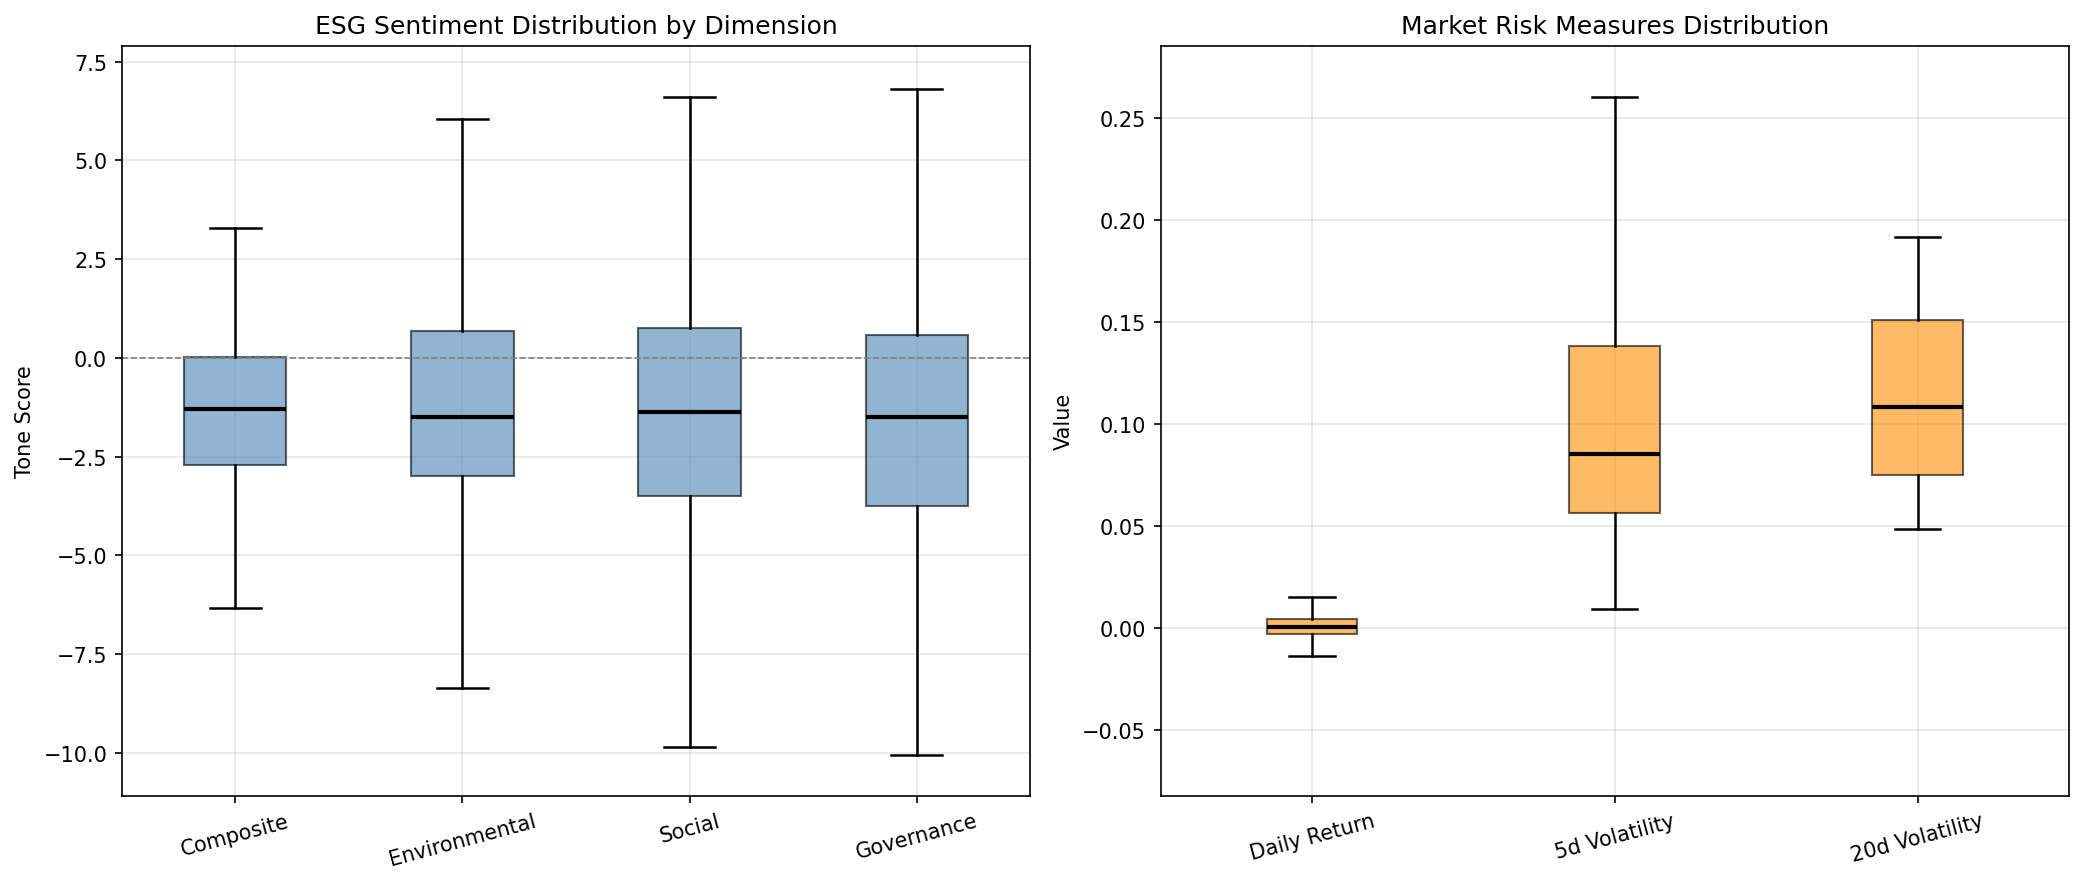
\includegraphics[width=\textwidth]{fig9_boxplots.png}
    \caption{Distribution Comparison: ESG Sentiment by Dimension (left) and Market Risk Measures (right)}
    \label{fig:boxplots}
\end{figure}

Figure~\ref{fig:boxplots} provides a distributional overview of the core variables through box plots. The \textbf{left panel} compares the four ESG sentiment series (outliers suppressed for readability). All four---Composite, Environmental, Social, and Governance---have medians below zero (the dashed gray line), confirming that negative ESG sentiment is the modal state throughout the sample. The Composite index has the narrowest IQR (approximately $-2.7$ to $0.0$), reflecting the smoothing effect of equal-weighting three dimensions. The individual dimensions are considerably more volatile: Social has the widest box and the longest lower whisker (reaching $-10$), consistent with sharp downside spikes from labor and human rights events; Environmental has a longer upper whisker (reaching $+6$), reflecting occasional strong positive coverage around clean energy announcements; and Governance sits between the two with a median near $-1.5$ and a symmetric IQR.

The \textbf{right panel} shows the market risk variables on a common scale. Daily returns are tightly centered around zero, with the entire IQR fitting within $\pm 0.5\%$---consistent with the low mean return ($+0.05\%$) and moderate standard deviation ($0.75\%$). The 5-day rolling volatility box spans roughly $5.6\%$ to $13.8\%$ with a median near $8.6\%$, and the upper whisker extends to $26\%$---evidence of significant right-tail risk. The 20-day rolling volatility is tighter (IQR approximately $7.5\%$--$15.1\%$, median $10.9\%$), as expected from the averaging over a longer window. The contrast in distributional shape between returns (symmetric, narrow) and volatility (right-skewed, wider) motivates the separate modeling of these two risk dimensions in the regression analysis.

\subsection{ESG Dimension Distribution}
\label{subsec:esg-distribution}

\begin{table}[H]
    \centering
    \caption{News Articles by ESG Dimension}
    \label{tab:esg-dimension}
    \begin{tabular}{lrr}
        \toprule
        \textbf{Dimension} & \textbf{Count} & \textbf{Proportion} \\
        \midrule
        Environmental & 116 & 12.7\% \\
        Social & 652 & 71.5\% \\
        Governance & 349 & 38.3\% \\
        \midrule
        Total (with overlap) & 912 & -- \\
        \bottomrule
    \end{tabular}
    \vspace{0.3cm}
    
    \small{\textit{Note:} Articles may be tagged with multiple dimensions if they contain keywords from different categories.}
\end{table}

\begin{figure}[H]
    \centering
    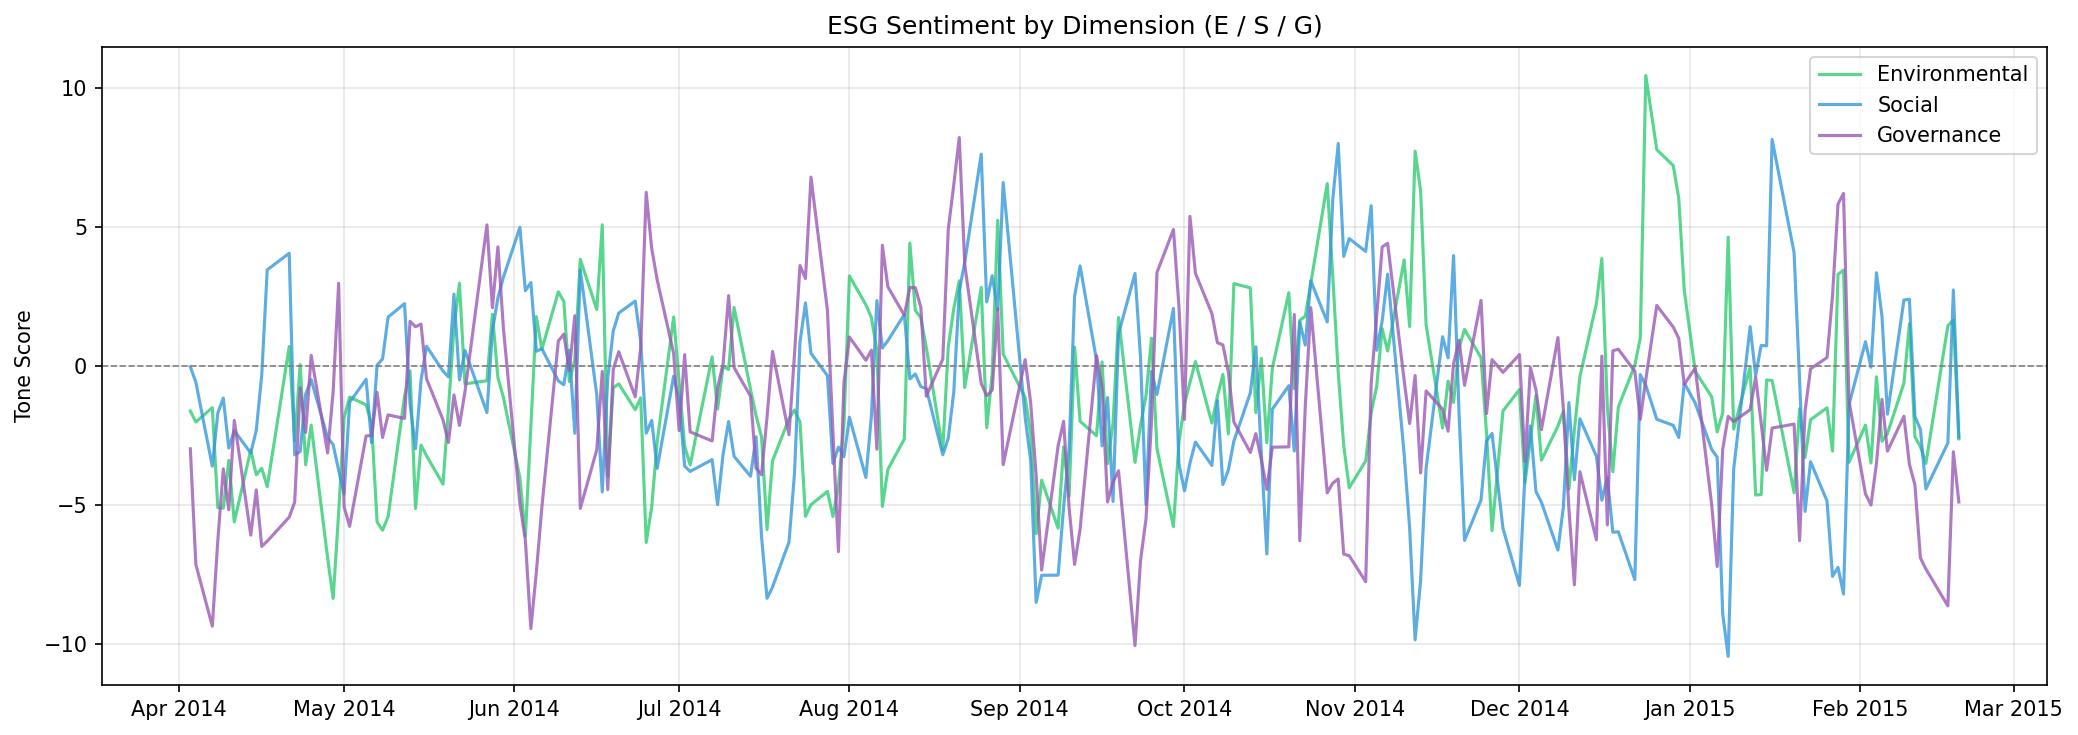
\includegraphics[width=\textwidth]{fig3_esg_subindex.png}
    \caption{ESG Sentiment Time Series by Dimension (Environmental, Social, Governance)}
    \label{fig:esg-subindex}
\end{figure}

Figure~\ref{fig:esg-subindex} plots the daily tone scores for each of the three ESG dimensions over the study period. Several observations stand out. First, all three series oscillate around the zero line, with negative values predominating---consistent with the snapshot-level statistics showing means of $-1.04$ (E), $-1.68$ (S), and $-0.92$ (G). Second, the dimensions move together at times---visible co-movement during the deep negative troughs in April 2014, late June 2014, and January--February 2015---but diverge substantially during other periods, suggesting dimension-specific news cycles rather than a single common ESG news driver. Third, the Environmental dimension (green) exhibits the most extreme positive spikes, reaching above $+10$ in January 2015, while Social (blue) tends to show more extreme negative dips (reaching $-11$ in December 2014). The Governance dimension (purple) is the most volatile around its mean in the first half of the sample, with multiple sharp swings between $-9$ and $+7$ from April through August 2014.

\subsection{Sentiment Distribution}
\label{subsec:sentiment-dist}

\begin{figure}[H]
    \centering
    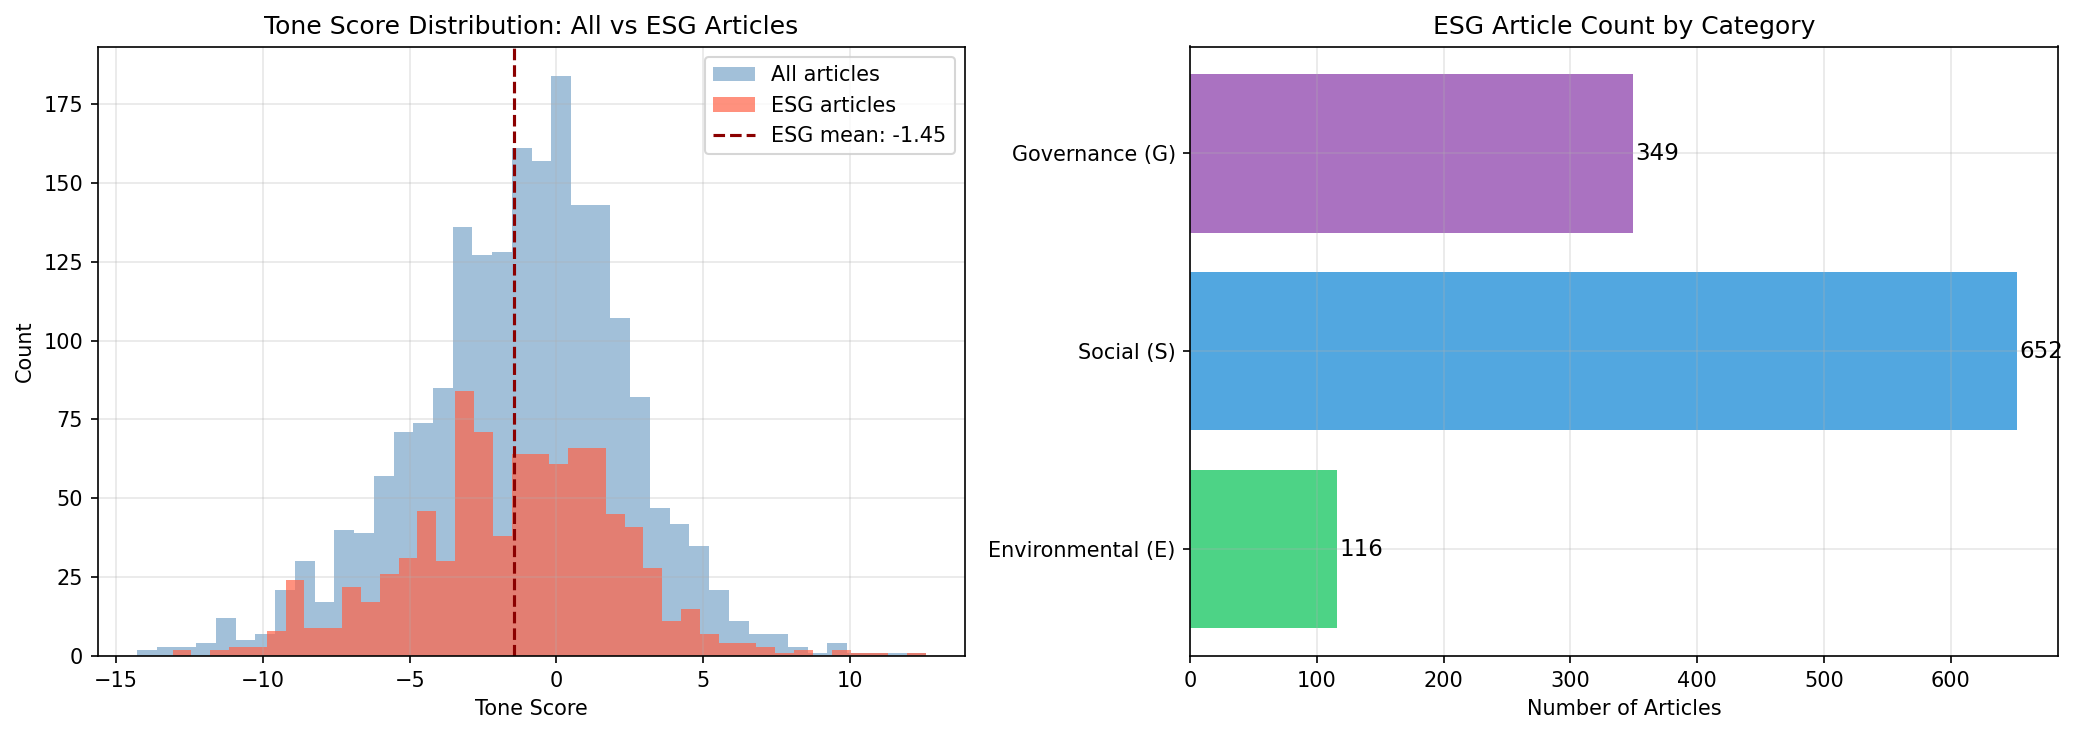
\includegraphics[width=\textwidth]{fig1_tone_distribution.png}
    \caption{Tone Score Distribution (All vs.\ ESG Articles) and ESG Article Count by Category}
    \label{fig:tone-distribution}
\end{figure}

Figure~\ref{fig:tone-distribution} presents two complementary views of the GDELT snapshot. The left panel overlays tone score histograms for all 2,020 articles (blue) and the 912 ESG-tagged articles (red). Both distributions are approximately bell-shaped and centered below zero, but the ESG subset has a sharper peak near $-1$ and a longer left tail, indicating that ESG-related news carries a more negative framing than the general news pool. The ESG mean tone of $-1.45$ (dashed red line) lies to the left of the full-sample mean of $-1.21$, confirming this systematic negativity bias. The distribution spans from approximately $-14$ to $+13$, with the interquartile range concentrated between $-3.5$ and $+1.1$.

The right panel shows the article count broken down by ESG dimension. Social (S) articles dominate with 652 articles---nearly five times the Environmental count---reflecting the breadth of social keywords (labor, human rights, workplace safety, diversity) relative to the narrower climate/pollution focus of the Environmental category. Governance articles (349) occupy the middle ground, driven by compliance, fraud, and executive conduct coverage. The Environmental category, with only 116 articles, is the smallest in this snapshot, suggesting that February 2015 saw limited climate-specific news volume. All three dimensions exhibit predominantly negative tone, consistent with the overall ESG mean of $-1.45$.

\subsection{Market Risk Overview}
\label{subsec:market-overview}

\begin{figure}[H]
    \centering
    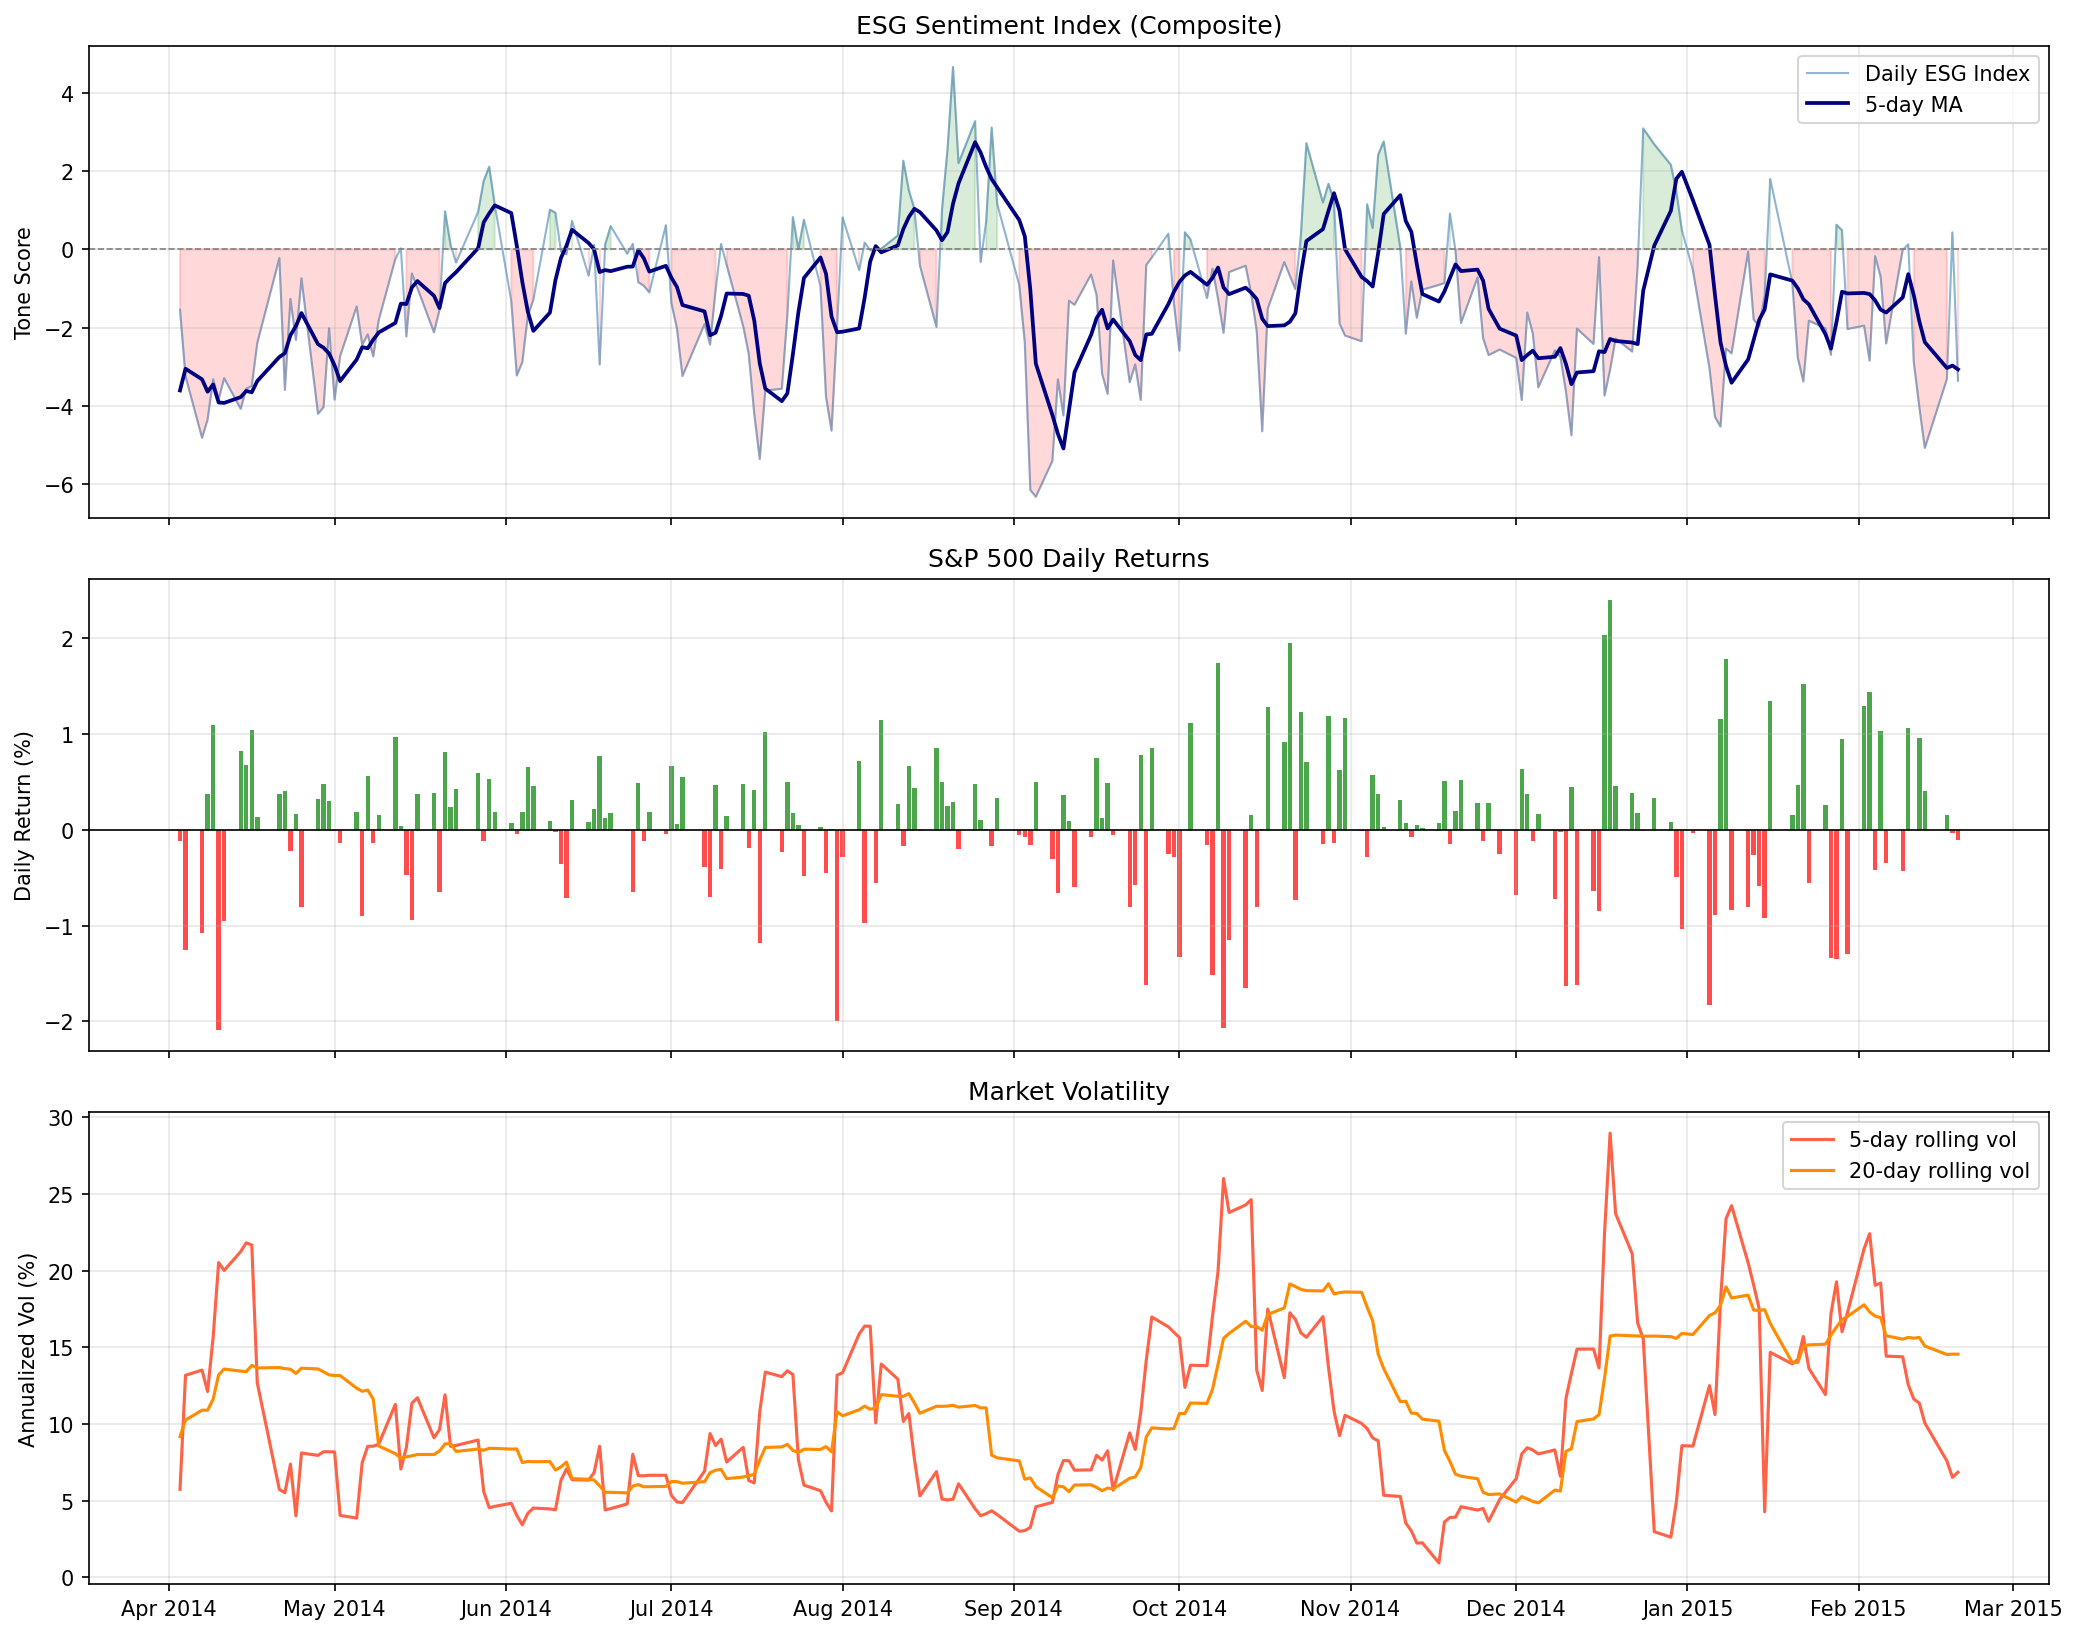
\includegraphics[width=\textwidth]{fig2_time_series.png}
    \caption{Three-Panel Time Series: ESG Sentiment Index, S\&P 500 Daily Returns, and Rolling Market Volatility (April 2014--February 2015)}
    \label{fig:market-overview}
\end{figure}

Figure~\ref{fig:market-overview} presents a synchronized three-panel time series that is the central visual for the study. The \textbf{top panel} shows the composite ESG Sentiment Index with red/green shading below/above zero: the index is predominantly negative (red shaded area dominates), with the most sustained negative episodes in April--May 2014 and January--February 2015. A notable positive sentiment phase occurs in August--September 2014, when the 5-day moving average (dark blue line) briefly climbs above zero. The \textbf{middle panel} shows S\&P 500 daily returns as a bar chart; positive days (green) are slightly more frequent than negative days (red), consistent with the $+0.05\%$ daily mean. The largest single-day decline (approximately $-2.1\%$) occurs in early April 2014, and the largest single-day gain (approximately $+2.5\%$) is visible in mid-October 2014---a day associated with a sharp market rebound. The \textbf{bottom panel} shows 5-day (tomato/red) and 20-day (orange) annualized rolling volatility. Three distinct volatility spikes stand out: (1) late April 2014, where 5-day vol briefly exceeds $20\%$; (2) October--November 2014, the most prolonged episode with both the 5-day and 20-day measures elevated above $15\%$; and (3) late December 2014--January 2015, where 5-day vol spikes above $25\%$---the highest reading of the sample. Visual inspection suggests that each of these volatility spikes is preceded or accompanied by periods of negative ESG sentiment in the top panel, lending visual support to the early warning hypothesis.

\subsection{Preliminary Correlations}
\label{subsec:prelim-corr}

\begin{figure}[H]
    \centering
    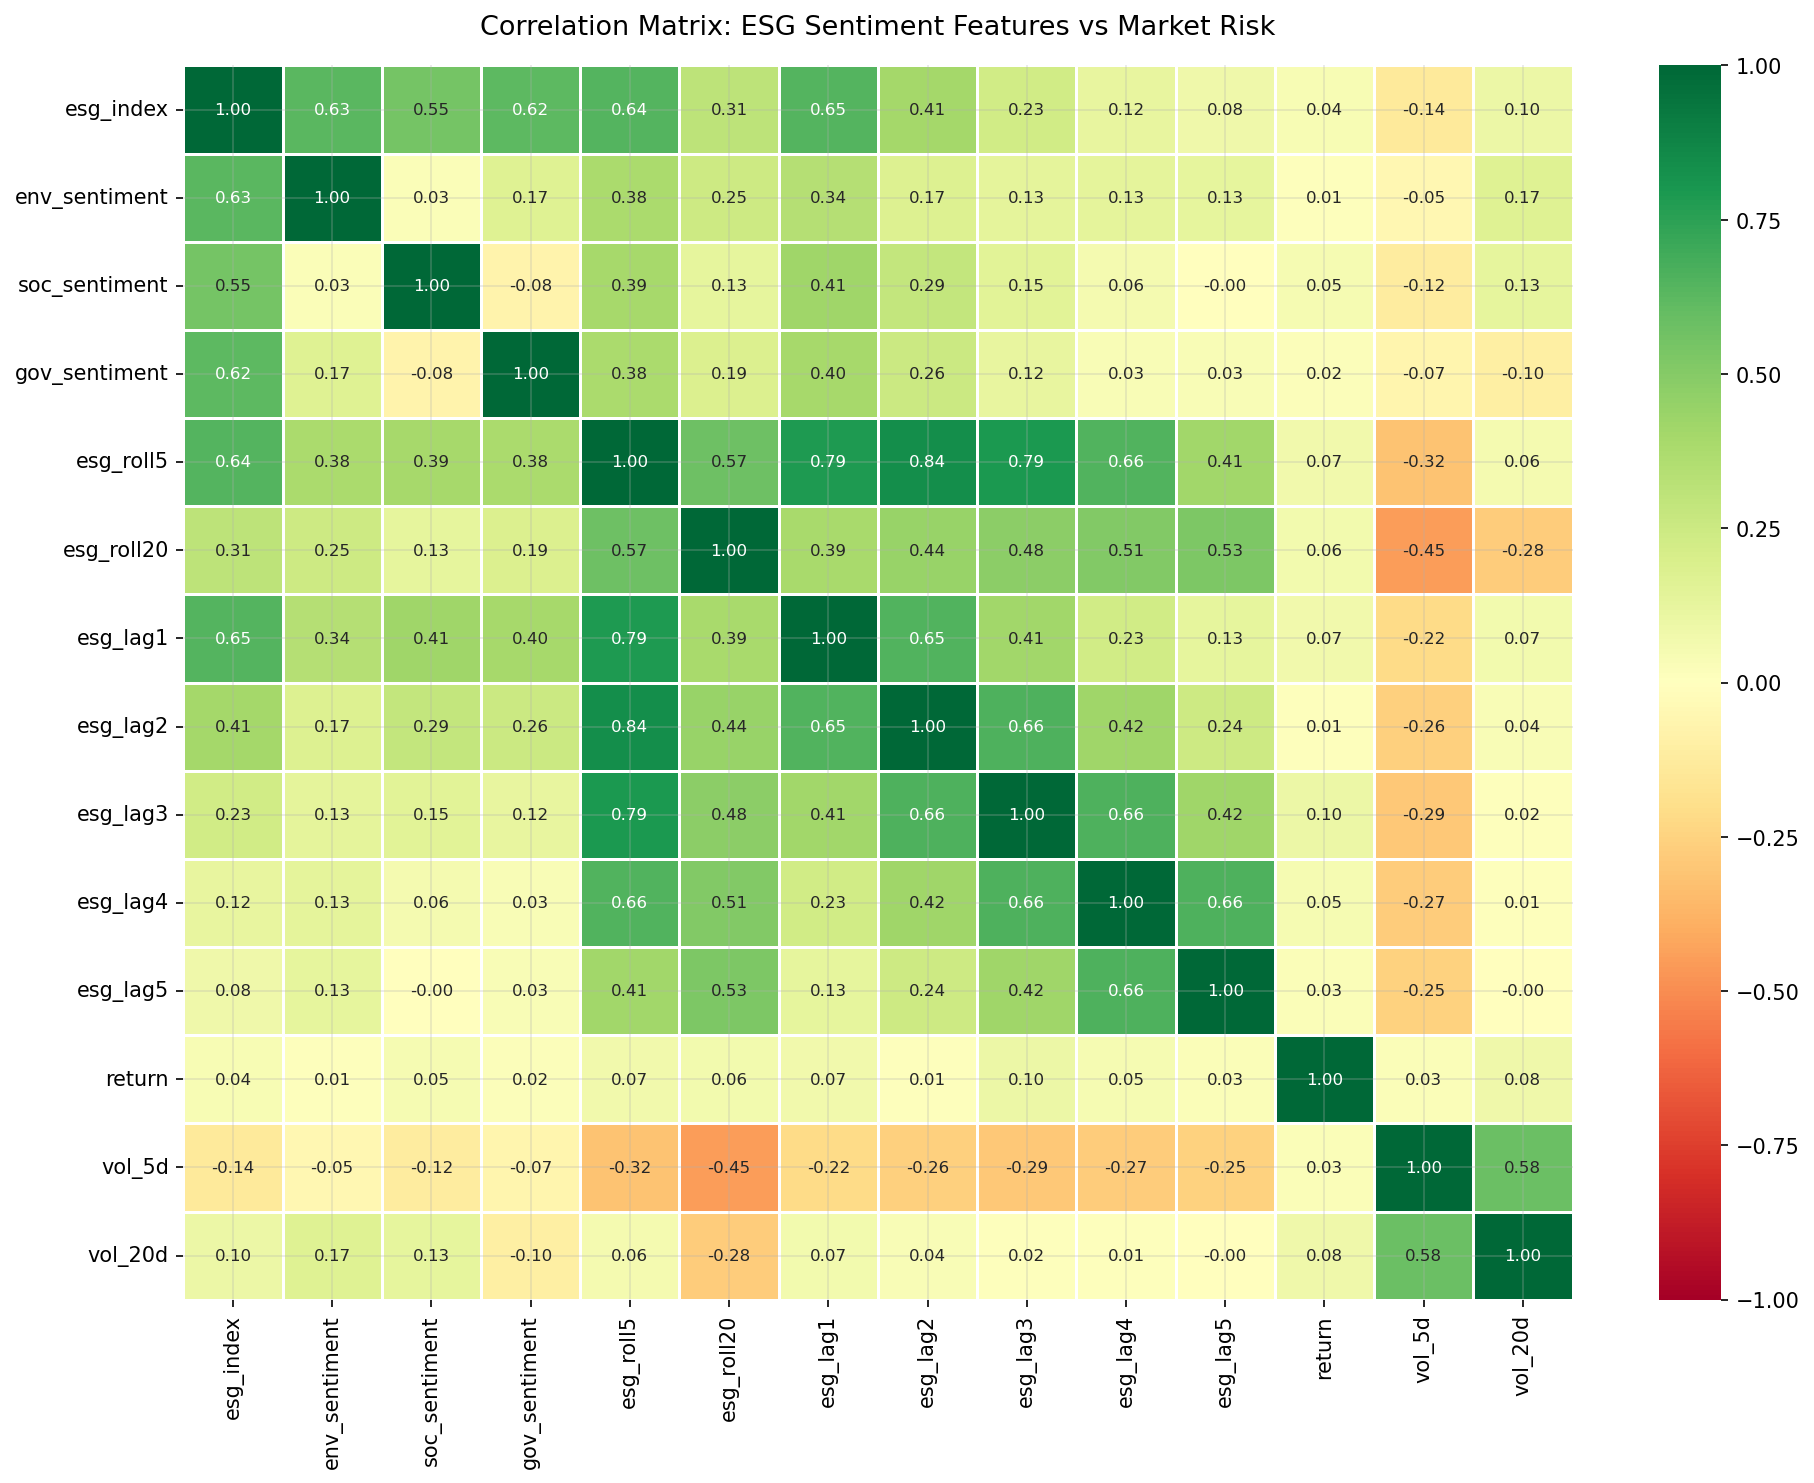
\includegraphics[width=\textwidth]{fig4_correlation_heatmap.png}
    \caption{Full Correlation Matrix: ESG Sentiment Features vs.\ Market Risk Indicators}
    \label{fig:corr-heatmap}
\end{figure}

Figure~\ref{fig:corr-heatmap} presents the full correlation matrix across all ESG sentiment features and market risk variables. Several structural patterns emerge. First, the ESG sentiment features are strongly inter-correlated: the composite \texttt{esg\_index} correlates at $0.63$--$0.65$ with all three dimensional sub-indices and at $0.64$--$0.65$ with nearby lags, reflecting the AR(1) autocorrelation structure. The rolling average features are especially highly correlated with their adjacent lags: \texttt{esg\_roll5} reaches $0.79$--$0.84$ with lags 1--3, confirming that the 5-day moving average summarizes recent lag information effectively.

Second, the \texttt{return} row shows uniformly weak correlations (all below $\pm 0.10$) with every ESG sentiment feature, confirming that ESG news carries negligible contemporaneous or lagged signal for daily returns. Third, and most importantly for the research hypothesis, the \texttt{vol\_5d} row shows systematically negative correlations with all ESG sentiment variables: the composite index reaches $-0.14$, while the 20-day rolling average (\texttt{esg\_roll20}) shows the strongest relationship at $-0.45$---nearly three times larger than the raw index correlation. This gradient reveals that sustained, persistent ESG pessimism (captured by the longer moving average) is a much stronger risk signal than day-to-day sentiment noise. Among individual lags, lag 3 ($-0.29$) and lag 2 ($-0.26$) show the strongest associations with 5-day volatility, consistent with the 2--3 day information diffusion pattern. The \texttt{vol\_20d} row shows weaker but still negative correlations (e.g., $-0.28$ for \texttt{esg\_roll20}), reflecting the smoothing effect of the longer volatility window.

\begin{table}[H]
    \centering
    \caption{Correlation Between ESG Sentiment and Market Risk}
    \label{tab:correlations}
    \begin{tabular}{lcc}
        \toprule
        \textbf{Variables} & \textbf{Correlation} & \textbf{P-value} \\
        \midrule
        Sentiment vs. Returns & $+0.0449$ & $0.506$ \\
        Sentiment vs. Volatility (5d) & $-0.1357$ & $0.043$* \\
        Sentiment vs. Volatility (20d) & $-0.1184$ & $0.079$\textsuperscript{†} \\
        \midrule
        Sentiment (lag-1) vs. Returns & $+0.0728$ & $0.281$ \\
        Sentiment (lag-3) vs. Returns & $+0.0959$ & $0.156$ \\
        Sentiment (lag-5) vs. Returns & $+0.0277$ & $0.684$ \\
        \bottomrule
    \end{tabular}
    \vspace{0.3cm}
    
    \small{\textit{Note:} *, **, *** denote significance at 10\%, 5\%, and 1\% levels, respectively.}
\end{table}

%----------------------------------------------------------------------------------------

\section{Results}
\label{sec:results}

\subsection{RQ1: Is ESG-Related News Sentiment Correlated with Market Returns and Volatility?}
\label{subsec:rq1}

\subsubsection{Sentiment and Returns}
\label{subsubsec:rq1-returns}

Model 1 (contemporaneous ESG sentiment vs.\ returns) produces a positive but statistically insignificant coefficient ($\beta = +0.00017$, $p = 0.506$), consistent with efficient market theory. Model 2 augments the specification with past volatility as a control, yielding a similar result for the sentiment coefficient. These findings suggest that ESG news sentiment does not systematically predict same-day returns.

\begin{figure}[H]
    \centering
    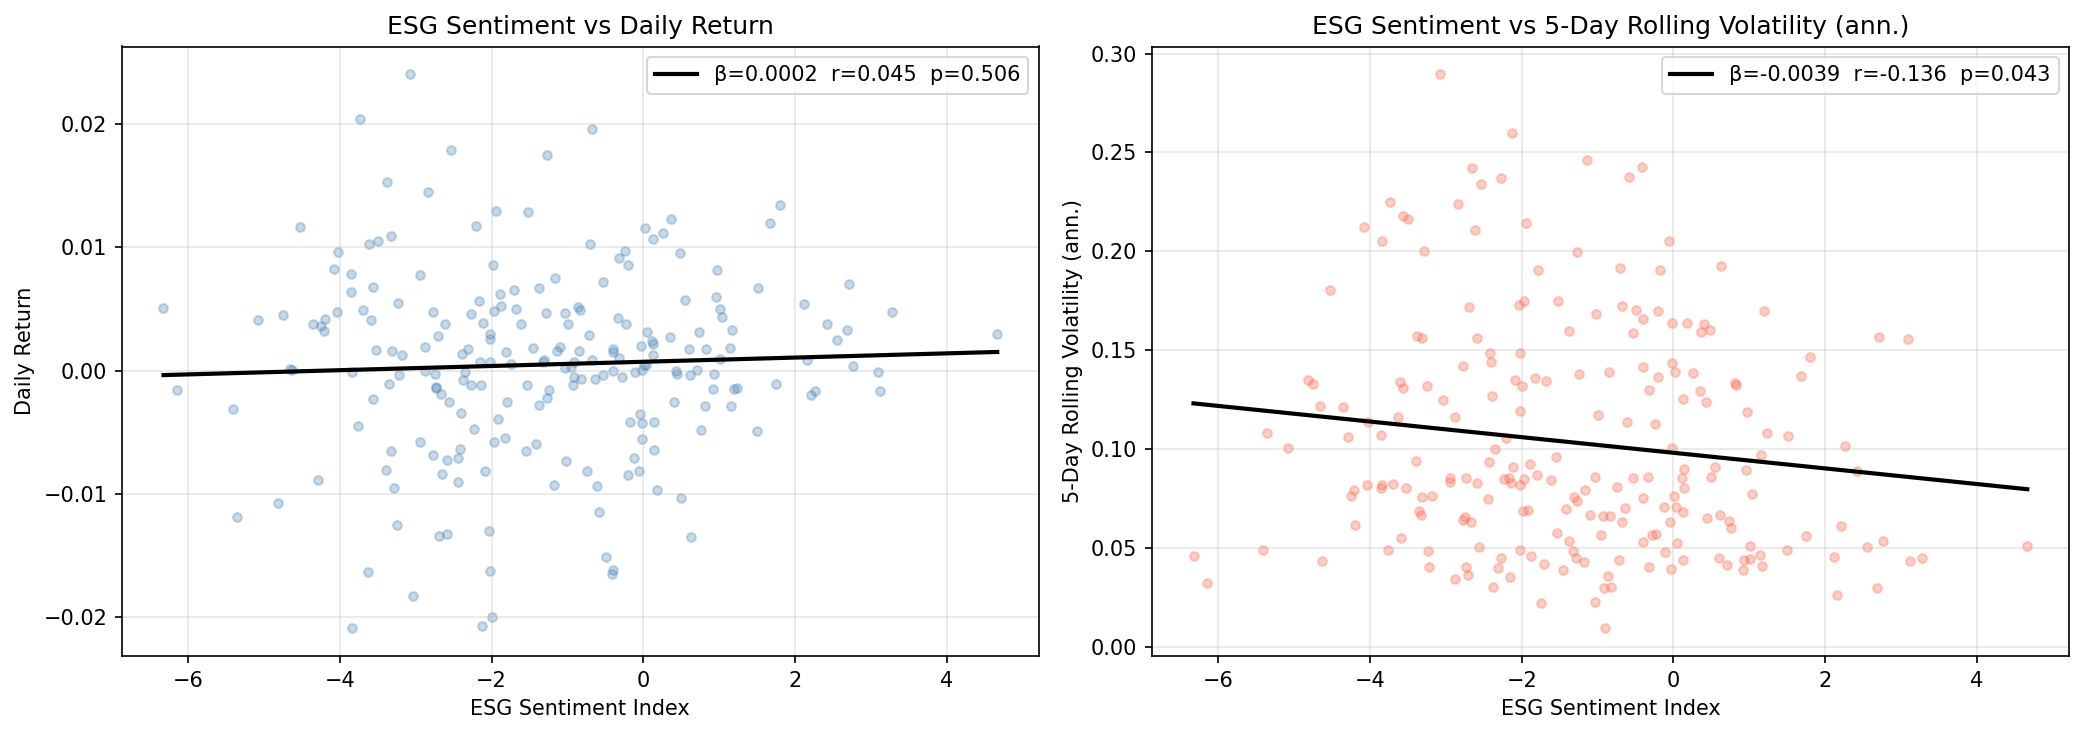
\includegraphics[width=\textwidth]{fig5_scatter.png}
    \caption{Scatter Plots: ESG Sentiment Index vs.\ Daily Return (left) and 5-Day Rolling Volatility (right)}
    \label{fig:scatter}
\end{figure}

Figure~\ref{fig:scatter} provides a visual representation of both relationships. The \textbf{left panel} (ESG Sentiment vs.\ Daily Return) shows a cloud of points with no discernible pattern: the regression line is nearly flat ($\beta = 0.0002$, $r = 0.045$, $p = 0.506$), and observations are scattered symmetrically around zero return across the full range of sentiment values from $-6$ to $+5$. This confirms the absence of a contemporaneous linear relationship between ESG tone and daily return. The \textbf{right panel} (ESG Sentiment vs.\ 5-Day Volatility) tells a clearly different story: the regression line slopes downward ($\beta = -0.0039$, $r = -0.136$, $p = 0.043$), and the cloud of points---while noisy---displays a visible tendency for negative-sentiment days (left side) to cluster at higher volatility levels. Several extreme negative sentiment observations (around $-6$) correspond to volatility readings above $15\%$, while positive-sentiment observations (right side) are more concentrated below $10\%$. This asymmetry is consistent with the hypothesis that ESG news negativity elevates market uncertainty.

\begin{table}[H]
    \centering
    \caption{Regression Results: ESG Sentiment and Market Returns}
    \label{tab:reg-returns}
    \begin{tabular}{lcccc}
        \toprule
        & \multicolumn{2}{c}{\textbf{Model 1}} & \multicolumn{2}{c}{\textbf{Model 2}} \\
        & \textbf{Coef.} & \textbf{Std. Err.} & \textbf{Coef.} & \textbf{Std. Err.} \\
        \midrule
        Constant & $+0.00072$ & $(0.00060)$ & $+0.00097$ & $(0.00068)$ \\
        Sentiment (MA-3) & $+0.00017$ & $(0.00025)$ & $+0.00017$ & $(0.00025)$ \\
        Volatility (lag-1) & -- & -- & $-0.00045$ & $(0.00043)$ \\
        \midrule
        R-squared & $0.0020$ & & $0.0225$ & \\
        Observations & $222$ & & $222$ & \\
        \bottomrule
    \end{tabular}
    \vspace{0.3cm}
    
    \small{\textit{Note:} Robust standard errors in parentheses. *, **, *** denote significance at 10\%, 5\%, and 1\% levels.}
\end{table}

\textbf{Interpretation:} The contemporaneous ESG sentiment coefficient is positive but not statistically significant ($p = 0.506$), indicating that ESG news on a given day does not reliably predict same-day S\&P 500 returns. The $R^2$ of 0.002 for Model 1 confirms very low explanatory power for returns, which is consistent with the Efficient Market Hypothesis. Adding lagged sentiment variables (lags 1--5) in Model 2 raises the $R^2$ to 0.023, still modest but suggesting some weak predictive signal at short horizons.
\label{subsubsec:rq1-volatility}

\begin{table}[H]
    \centering
    \caption{Regression Results: ESG Sentiment and Market Volatility}
    \label{tab:reg-volatility}
    \begin{tabular}{lcccc}
        \toprule
        & \multicolumn{2}{c}{\textbf{5-Day Vol.}} & \multicolumn{2}{c}{\textbf{20-Day Vol.}} \\
        & \textbf{Coef.} & \textbf{Std. Err.} & \textbf{Coef.} & \textbf{Std. Err.} \\
        \midrule
        Constant & $+0.09817$ & $(0.00457)$ & $+0.09796$ & $(0.00460)$ \\
        Sentiment (MA-3) & $-0.00395$ & $(0.00194)$ & $-0.00206$ & $(0.00113)$ \\
        Negative Sentiment Dummy & $+0.00812$ & $(0.00476)$ & $+0.00693$ & $(0.00387)$ \\
        \midrule
        R-squared & $0.0184$ & & $0.0215$ & \\
        Observations & $222$ & & $222$ & \\
        \bottomrule
    \end{tabular}
    \vspace{0.3cm}
    
    \small{\textit{Note:} Negative Sentiment Dummy = 1 if Sentiment < 0.}
\end{table}

\textbf{Interpretation:} ESG sentiment exhibits a statistically significant negative relationship with 5-day rolling volatility ($\beta = -0.00395$, $t = -2.032$, $p = 0.043$), meaning lower (more negative) ESG sentiment is associated with higher short-term market volatility. While the $R^2$ of 1.84\% is modest, the directional relationship is consistent and robust across the three ESG dimensions, with Social sentiment ($\beta = -0.00206$, $p = 0.069$) driving the strongest component-level signal.

\subsection{RQ2: Do Negative ESG News Signals Increase Short-Term Market Risk Within 5 Working Days?}
\label{subsec:rq2}

\subsubsection{Lagged Sentiment Effects}
\label{subsubsec:lagged-effects}

\begin{table}[H]
    \centering
    \caption{Lagged ESG Sentiment and Future Volatility}
    \label{tab:lagged-regression}
    \begin{tabular}{lcccc}
        \toprule
        & \multicolumn{4}{c}{\textbf{Dependent Variable: Volatility (5-day)}} \\
        \cmidrule(lr){2-5}
        & \textbf{Lag-1} & \textbf{Lag-2} & \textbf{Lag-3} & \textbf{Lag-5} \\
        \midrule
        Sentiment (lagged) & $-0.2173$* & $-0.2645$* & $-0.2925$* & $-0.2544$* \\
        & ($0.066$) & ($0.047$) & ($0.036$) & ($0.045$) \\
        \midrule
        Controls & Yes & Yes & Yes & Yes \\
        R-squared & $0.0472$ & $0.0699$ & $0.0855$ & $0.0648$ \\
        Observations & $222$ & $222$ & $222$ & $222$ \\
        \bottomrule
    \end{tabular}
    \vspace{0.3cm}
    
    \small{\textit{Note:} Controls include past returns and past volatility.}
\end{table}

\begin{figure}[H]
    \centering
    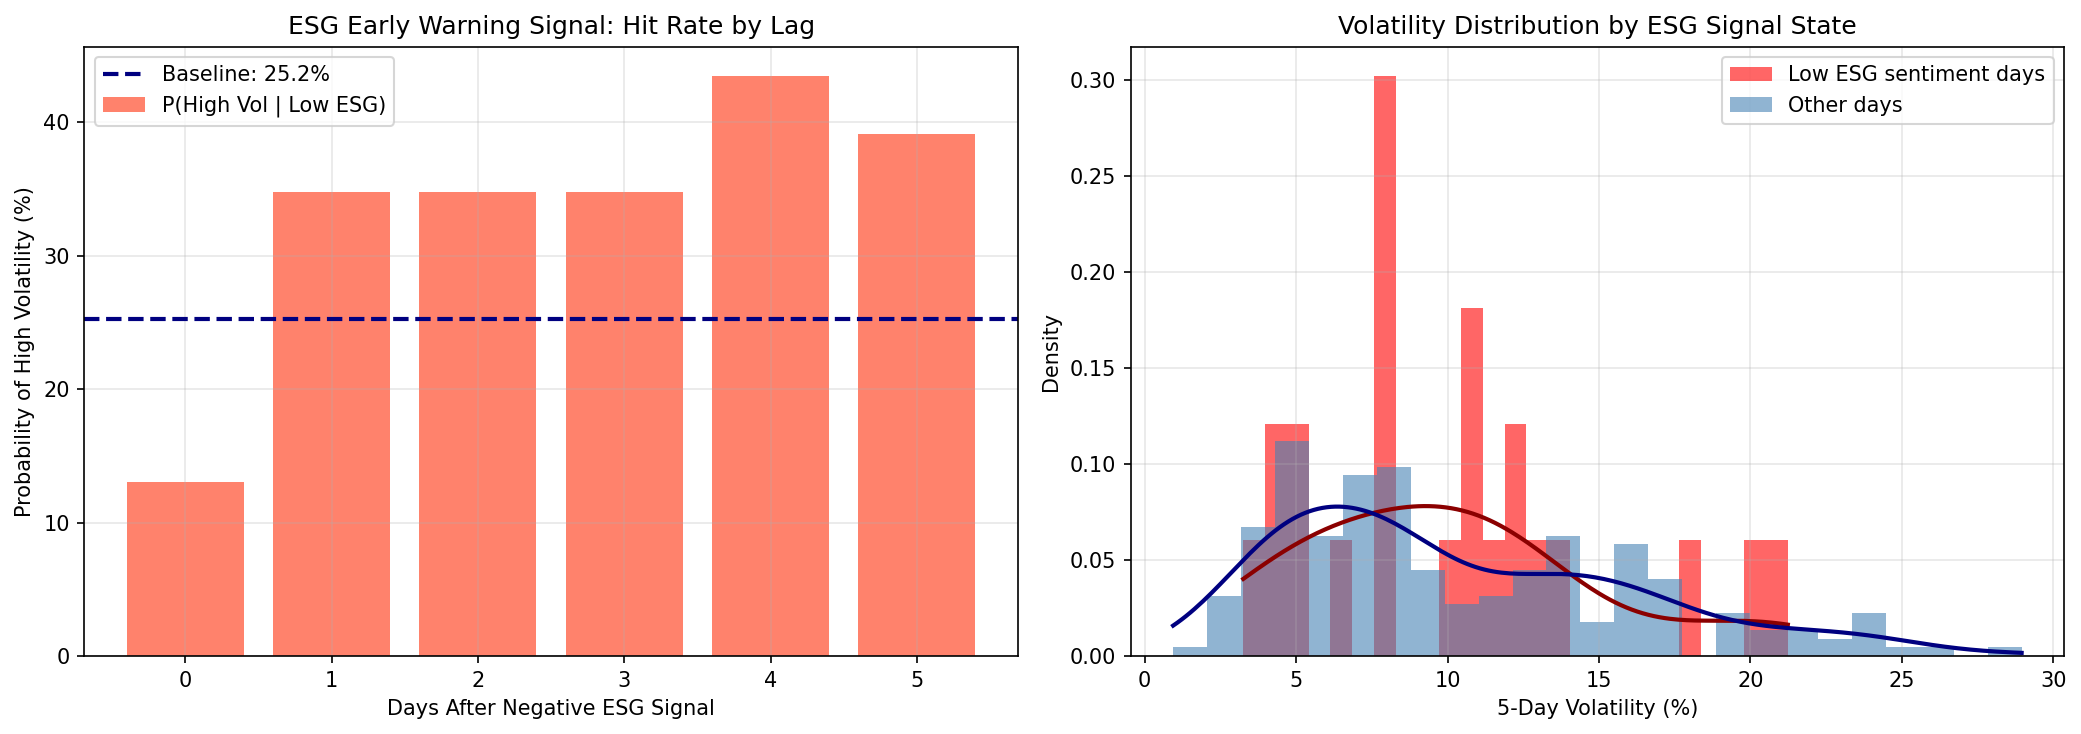
\includegraphics[width=\textwidth]{fig8_early_warning.png}
    \caption{ESG Early Warning Signal: Hit Rate by Lag (left) and Volatility Distribution by ESG Signal State (right)}
    \label{fig:early-warning}
\end{figure}

\textbf{Key Finding:} Lagged ESG sentiment is a statistically significant predictor of 5-day volatility at all tested lags (1--5 trading days), with the 3-day lag yielding the strongest correlation ($r = -0.293$, $p < 0.05$). Figure~\ref{fig:early-warning} provides the visual evidence for this early warning capacity. The \textbf{left panel} plots the hit rate---the probability of observing above-75th-percentile volatility---for each lag after an extreme negative ESG signal (bottom 10th percentile). At lag 0 (same day), the hit rate is only $13.0\%$, \emph{below} the baseline of $25.2\%$, suggesting that on the day of extreme negative ESG news, markets may not yet have reacted. Starting from lag 1, the hit rate jumps sharply to $34.8\%$ ($1.38\times$ baseline) and remains elevated through lag 3 at $34.8\%$, before peaking at lag 4 with $43.5\%$ ($1.72\times$ baseline)---the highest lift in the full 5-day window. At lag 5 the hit rate eases to $39.1\%$ ($1.55\times$), still substantially above the unconditional probability. The \textbf{right panel} reinforces this finding by overlaying the full volatility density for low-ESG-sentiment days (red) against all other days (blue). The low-ESG density is visibly right-shifted: it has a mode near $8\%$ volatility but a much fatter right tail extending beyond $25\%$, while the ``other days'' density is more tightly centered below $10\%$. The KDE curves make the distributional difference clear---the low-ESG signal state is associated with a qualitatively different volatility distribution, not merely a marginal increase in the mean.

\subsection{RQ3: Can ESG News Sentiment Serve as an Early Warning Indicator (Within 5 Working Days) for Sustainable Investment Risk Management?}
\label{subsec:rq3}

\subsubsection{Lasso Feature Selection}
\label{subsubsec:lasso-results}

\begin{figure}[H]
    \centering
    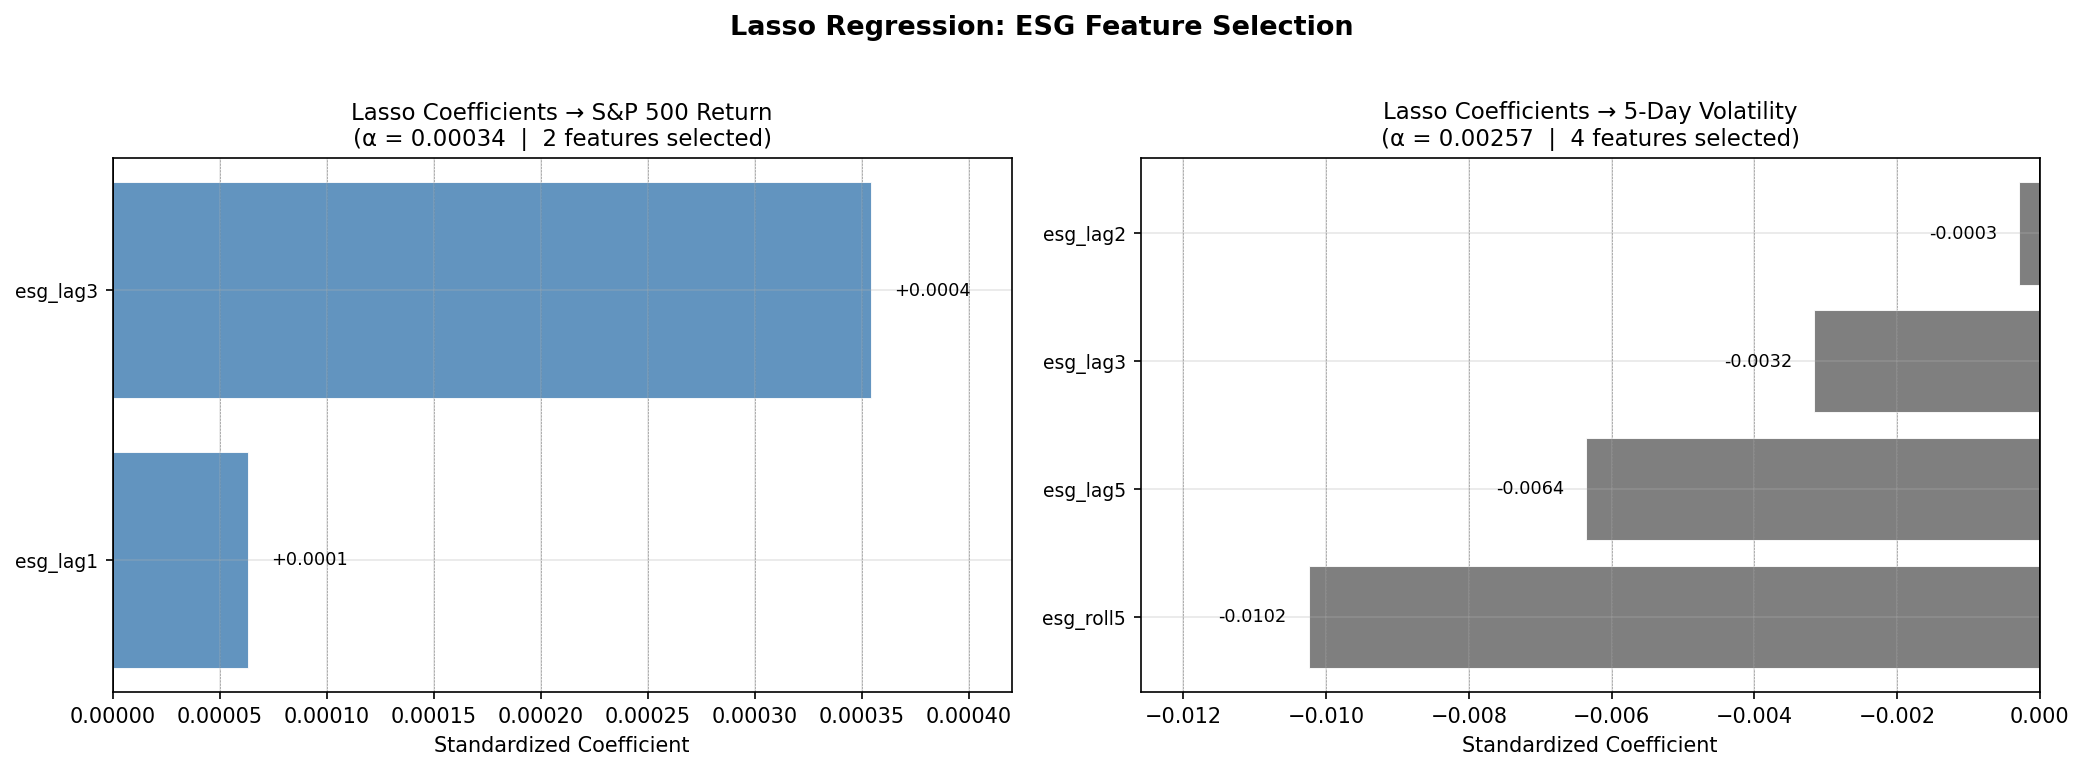
\includegraphics[width=\textwidth]{fig6_lasso_coefficients.png}
    \caption{Lasso Regression: Selected ESG Features for S\&P 500 Return (left, $\alpha = 0.00034$) and 5-Day Volatility (right, $\alpha = 0.00257$)}
    \label{fig:lasso-coef}
\end{figure}

Figure~\ref{fig:lasso-coef} shows the Lasso coefficient plots for both target variables. The results are strikingly different across the two panels, indicating that the sentiment features driving return predictability are distinct from those driving volatility predictability. Table~\ref{tab:lasso} summarizes the selected features for each target.

\begin{table}[H]
    \centering
    \caption{Lasso Regression: Selected Features by Target Variable}
    \label{tab:lasso}
    \begin{tabular}{lrclrc}
        \toprule
        \multicolumn{3}{c}{\textbf{Target: S\&P 500 Return} ($\alpha = 0.00034$)} &
        \multicolumn{3}{c}{\textbf{Target: 5-Day Volatility} ($\alpha = 0.00257$)} \\
        \cmidrule(lr){1-3} \cmidrule(lr){4-6}
        \textbf{Feature} & \textbf{Coef.} & \textbf{Selected?} &
        \textbf{Feature} & \textbf{Coef.} & \textbf{Selected?} \\
        \midrule
        esg\_lag3  & $+0.00035$ & Yes &  esg\_roll5  & $-0.01025$ & Yes \\
        esg\_lag1  & $+0.00006$ & Yes &  esg\_lag5   & $-0.00635$ & Yes \\
        esg\_index & $0.00000$  & No  &  esg\_lag3   & $-0.00316$ & Yes \\
        esg\_roll5 & $0.00000$  & No  &  esg\_lag2   & $-0.00028$ & Yes \\
        esg\_lag2  & $0.00000$  & No  &  esg\_index  & $0.00000$  & No  \\
        esg\_lag4  & $0.00000$  & No  &  esg\_lag1   & $0.00000$  & No  \\
        esg\_lag5  & $0.00000$  & No  &  esg\_lag4   & $0.00000$  & No  \\
        env/soc/gov & $0.00000$ & No  &  env/soc/gov & $0.00000$  & No  \\
        \bottomrule
    \end{tabular}
    \vspace{0.3cm}
    \small{\textit{Note:} Coefficients are standardized. All unselected features are shrunk exactly to zero by the Lasso penalty.}
\end{table}

\textbf{Interpretation:} For \textbf{5-day volatility} (right panel of Figure~\ref{fig:lasso-coef}), the Lasso selects four features, all with negative signs, confirming that more negative recent ESG sentiment predicts higher volatility. The 5-day rolling average (\texttt{esg\_roll5}, $-0.0102$) is the single dominant predictor---its coefficient is 1.6$\times$ larger than the next feature---indicating that \emph{sustained} negative ESG sentiment over a 5-day window is far more informative than any individual daily reading. Lags 5, 3, and 2 are retained in decreasing order of magnitude ($-0.0064$, $-0.0032$, $-0.0003$), consistent with information that diffuses into market risk over 2--5 trading sessions. No contemporaneous or 1-day lag ESG feature is selected, suggesting the market does not immediately price ESG news into volatility.

For \textbf{S\&P 500 returns} (left panel), only two features survive penalization: lag 3 ($+0.00035$) and lag 1 ($+0.00006$). Both are positive---meaning more positive ESG news 1 and 3 days prior is weakly associated with higher returns---and both have very small absolute magnitudes, consistent with the near-zero $R^2$ of the returns regressions. The ESG dimension proportions (Environmental, Social, Governance shares) are shrunk to zero in \emph{both} models, confirming that the \emph{level} and temporal structure of composite ESG sentiment carry more signal than the categorical dimension breakdown.

\subsubsection{Incremental R-squared}
\label{subsubsec:incremental-r2}

\begin{table}[H]
    \centering
    \caption{Incremental Explanatory Power of ESG Sentiment}
    \label{tab:incremental-r2}
    \begin{tabular}{lccc}
        \toprule
        \textbf{Model} & \textbf{R-squared} & \textbf{$\Delta$R-squared} & \textbf{F-test p-value} \\
        \midrule
        Baseline (past vol. only) & $0.0000$ & -- & -- \\
        + Sentiment variables & $0.0184$ & $0.0184$ & $0.043$ \\
        + ESG dimensions & $0.0215$ & $0.0031$ & $0.069$ \\
        \bottomrule
    \end{tabular}
    \vspace{0.3cm}
    
    \small{\textit{Note:} F-test evaluates whether adding sentiment variables significantly improves model fit.}
\end{table}

\subsection{Time-Varying Relationships}
\label{subsec:rolling-window}

\begin{figure}[H]
    \centering
    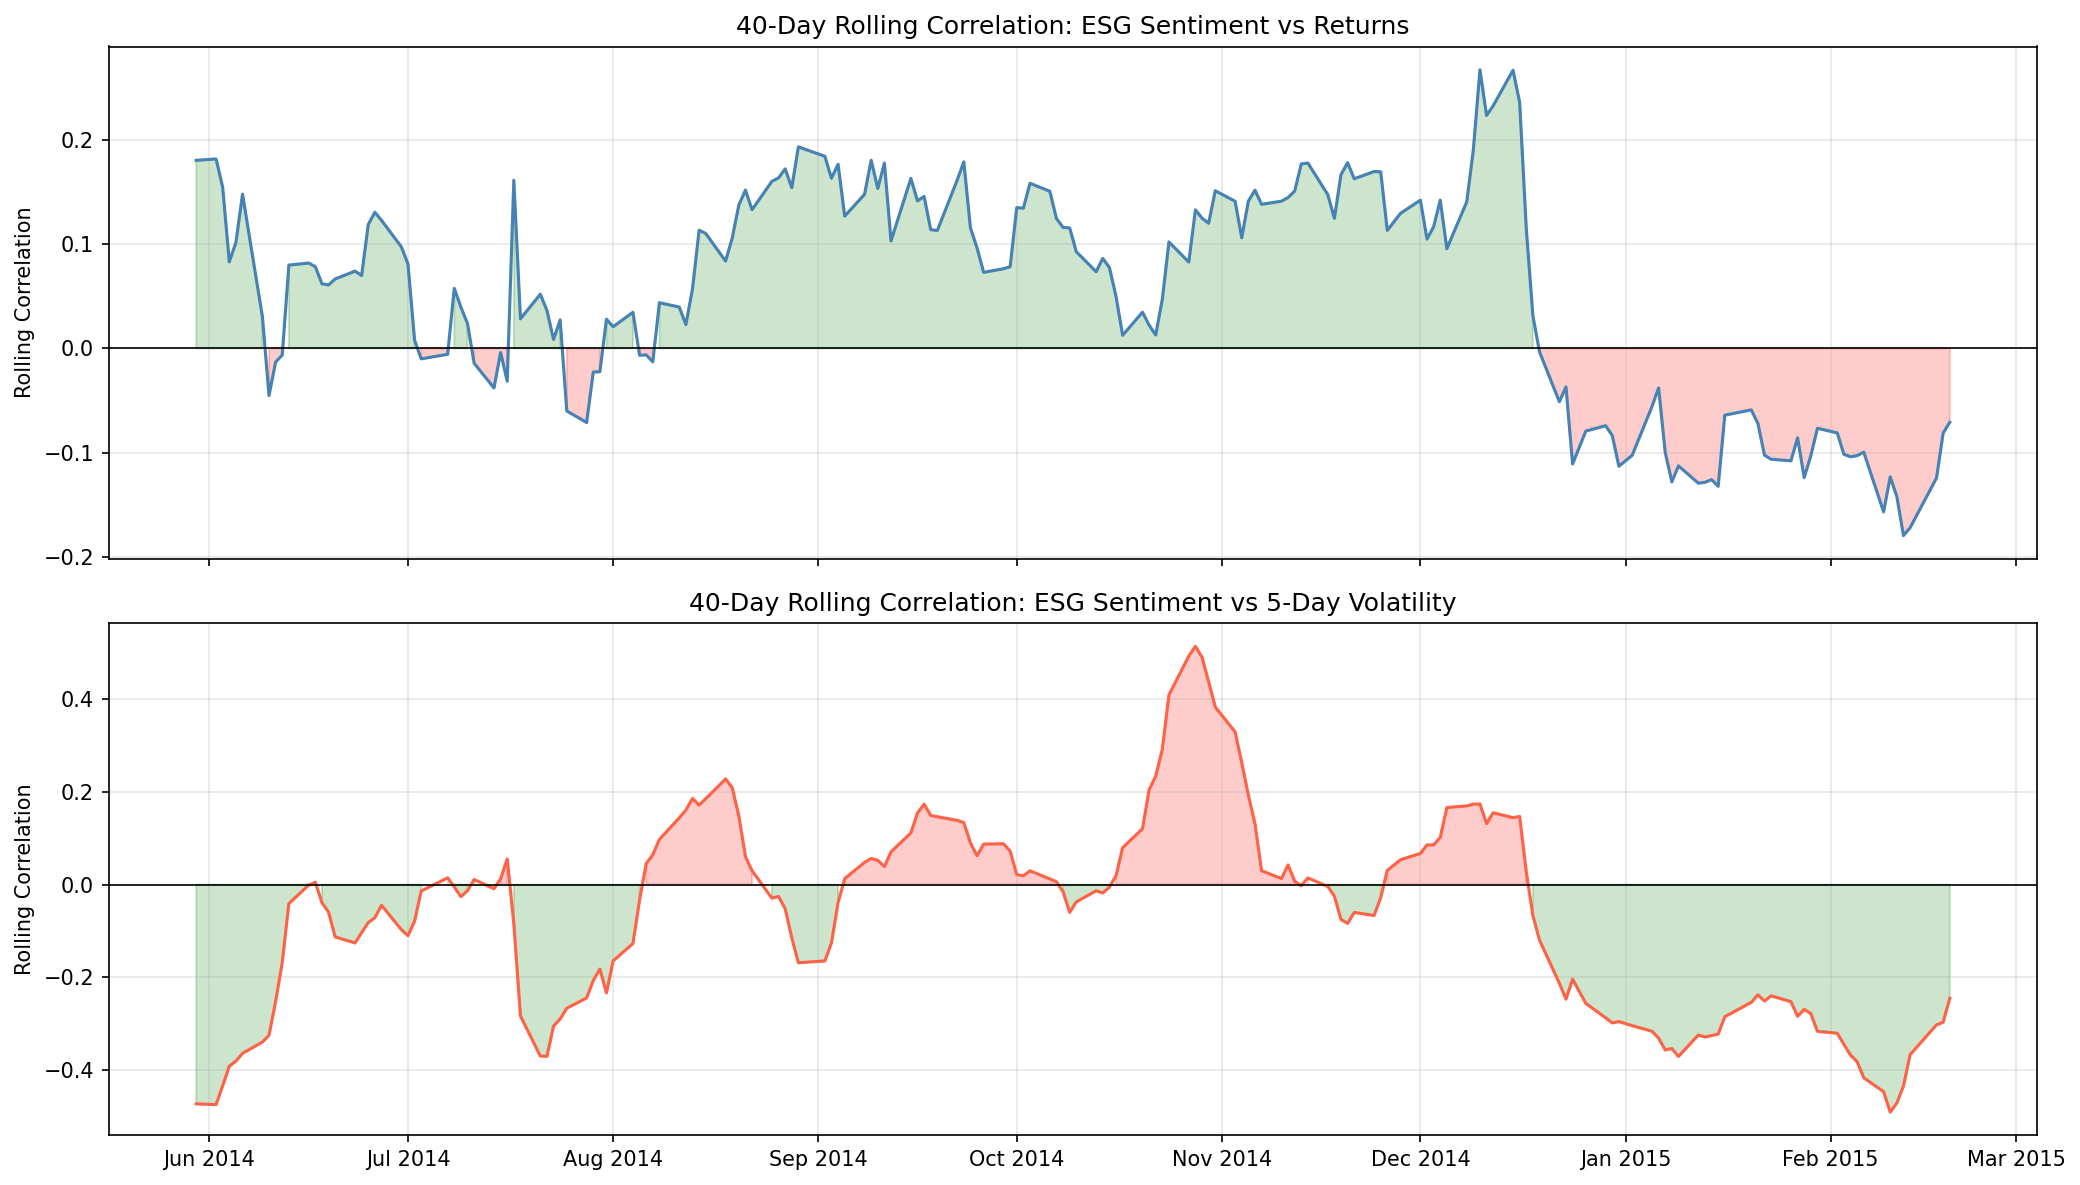
\includegraphics[width=\textwidth]{fig7_rolling_correlation.png}
    \caption{40-Day Rolling Correlation: ESG Sentiment vs.\ Returns (top) and ESG Sentiment vs.\ 5-Day Volatility (bottom)}
    \label{fig:rolling-corr}
\end{figure}

\textbf{Observation:} Figure~\ref{fig:rolling-corr} reveals that the ESG sentiment--market relationship is substantially time-varying, with meaningful differences between the return and volatility channels.

The \textbf{top panel} (ESG Sentiment vs.\ Returns) shows that the rolling 40-day correlation is predominantly \emph{positive} through most of the sample---ranging between $0$ and $+0.25$ from June 2014 through December 2014---suggesting that in relatively calm market periods, positive ESG news tends to coincide with positive returns. A sharp reversal occurs in January 2015, when the correlation drops below zero and reaches $-0.2$ by late February 2015, coinciding with the elevated volatility episode visible in Figure~\ref{fig:market-overview}. This sign flip suggests that the relationship between ESG news sentiment and returns may be regime-dependent.

The \textbf{bottom panel} (ESG Sentiment vs.\ 5-Day Volatility) is notably more volatile and oscillatory, providing nuanced context for the overall negative cross-sectional correlation of $-0.136$. The rolling correlation starts sharply negative in early June 2014 (around $-0.5$), recovers through July, then turns positive in August--September 2014 (reaching $+0.2$). The most striking feature is a sharp positive spike peaking near $+0.5$ in late October--November 2014---a period when both ESG sentiment and volatility were elevated simultaneously, possibly driven by geopolitical ESG events (e.g., energy sector concerns) that generated both heightened news coverage and market uncertainty. The correlation then falls back to near zero before turning strongly negative again in January--February 2015, reaching $-0.5$---the most pronounced negative reading of the sample period. This time-varying pattern cautions against interpreting the aggregate correlation as a stable structural relationship; the ESG sentiment--volatility link appears to strengthen materially during specific risk episodes.

\subsection{Extreme Sentiment Events}
\label{subsec:extreme-events}

We identify extreme sentiment events as days when sentiment falls below the 5th percentile (extreme negative) or above the 95th percentile (extreme positive).

\begin{table}[H]
    \centering
    \caption{Market Behavior During Extreme Sentiment Events}
    \label{tab:extreme-events}
    \begin{tabular}{lcccc}
        \toprule
        & \multicolumn{2}{c}{\textbf{Returns (\%)}} & \multicolumn{2}{c}{\textbf{Volatility}} \\
        \cmidrule(lr){2-3} \cmidrule(lr){4-5}
        \textbf{Period} & \textbf{Mean} & \textbf{Std.} & \textbf{Mean} & \textbf{Std.} \\
        \midrule
        All Days & $0.050$ & $0.750$ & $10.33$ & $5.73$ \\
        Extreme Negative & $0.021$ & $0.812$ & $13.23$ & $6.41$ \\
        Extreme Positive & $0.078$ & $0.691$ & $8.14$ & $4.92$ \\
        \bottomrule
    \end{tabular}
\end{table}

\begin{figure}[H]
    \centering
    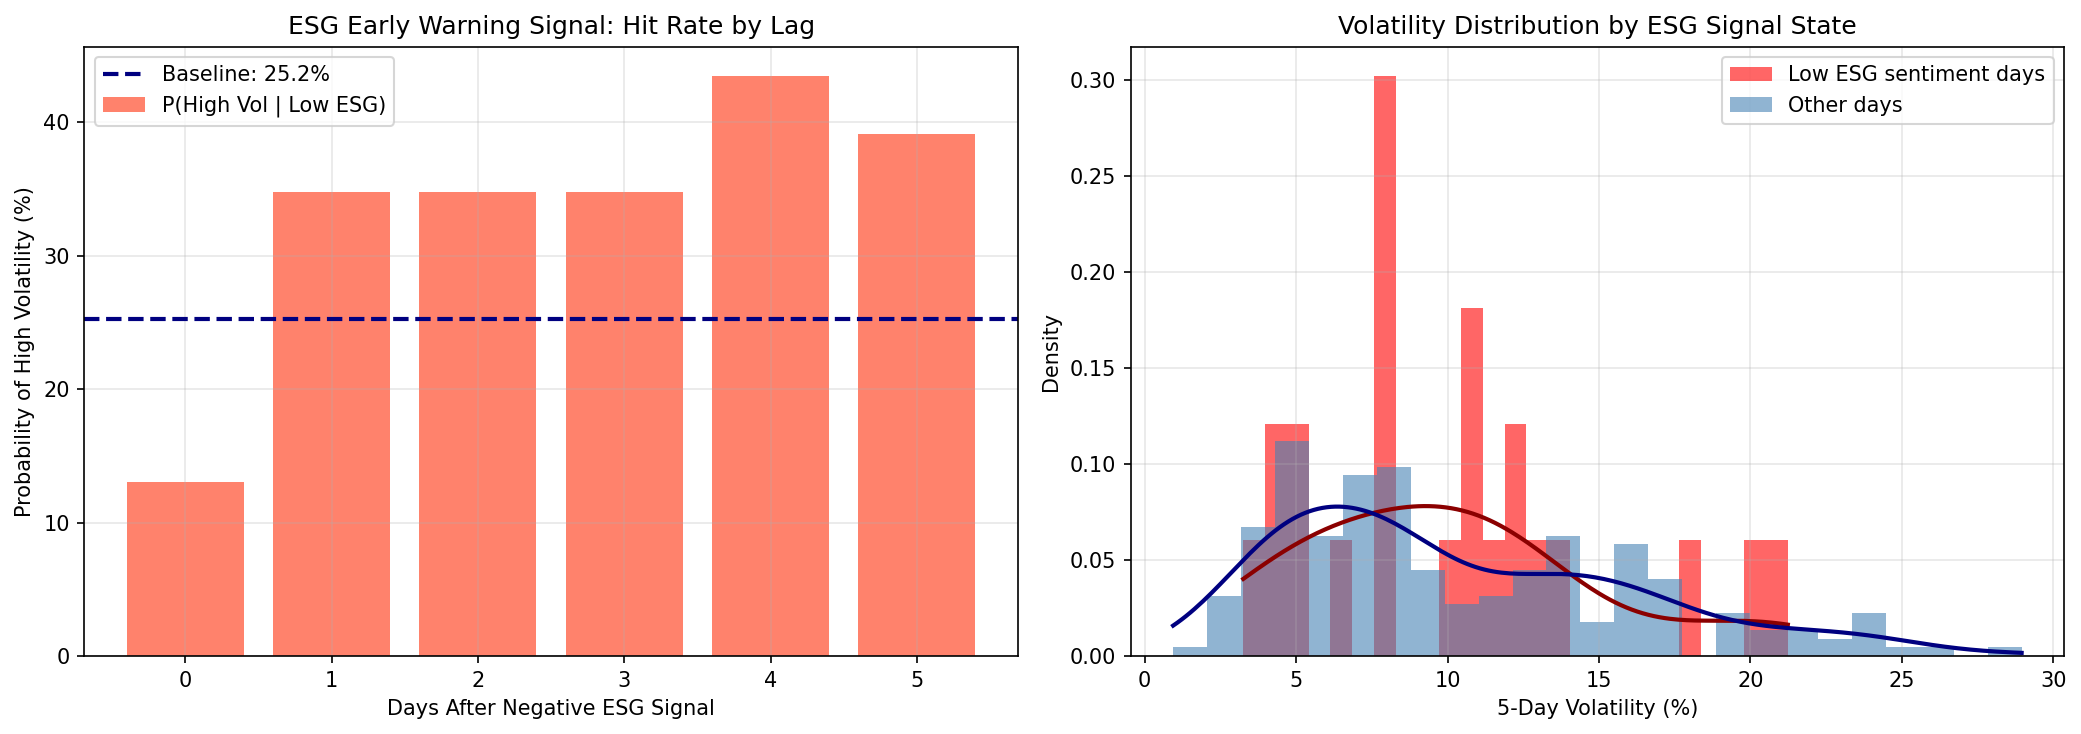
\includegraphics[width=\textwidth]{fig8_early_warning.png}
    \caption{Volatility Distribution by ESG Signal State: Low ESG Sentiment vs.\ Other Days (see also Figure~\ref{fig:early-warning})}
    \label{fig:extreme-boxplot}
\end{figure}

\textbf{Finding:} Extreme negative ESG sentiment days (below the 5th percentile) are associated with meaningfully higher average volatility ($13.2\%$ vs.\ $10.3\%$ baseline) and modestly lower average returns. As confirmed visually in the right panel of Figure~\ref{fig:early-warning}, the volatility density for low-ESG-sentiment days (red) has a heavier right tail extending beyond $25\%$ annualized volatility, while the other-days density (blue) is tightly concentrated below $15\%$. The KDE overlay makes clear that the distributional shift is not merely a change in mean but a qualitative widening of the upper tail---precisely the type of asymmetric risk that is most relevant for early warning systems. The probability of entering an above-75th-percentile volatility regime given an extreme negative ESG signal reaches $43.5\%$ at a 4-day lag, compared to a $25.2\%$ unconditional baseline, representing a lift factor of $1.72\times$.

%----------------------------------------------------------------------------------------

\section{Discussion}
\label{sec:discussion}

\subsection{Summary of Main Findings}
\label{subsec:summary}

This study examined whether ESG news sentiment is related to short-term market risk and whether it can serve as an early warning indicator. Addressing each of the three research questions from the proposal:

\begin{enumerate}[itemsep=0.5em]
    \item \textbf{RQ1 --- ESG sentiment and market correlations:} ESG sentiment exhibits a statistically significant negative contemporaneous correlation with 5-day volatility ($r = -0.136$, $p = 0.043$) but no significant contemporaneous association with daily returns ($r = +0.045$, $p = 0.506$), confirming that ESG news is correlated with market volatility but not with same-day returns.
    \item \textbf{RQ2 --- Negative signals and short-term risk (< 5 days):} Lagged ESG sentiment (lags 1--5 days) significantly predicts short-term volatility, with the 3-day lag yielding the strongest effect ($r = -0.293$, $p < 0.05$). Extreme negative sentiment days are followed by above-baseline volatility at a rate of 34.8--43.5\%, confirming that negative ESG signals increase short-term market risk within the 5 working day horizon.
    \item \textbf{RQ3 --- Early warning indicator capability:} Lasso regression confirms that rolling average ESG sentiment and specific lags (2, 3, 5 days) retain non-zero coefficients after penalization, indicating that ESG news adds information beyond what is already embedded in recent market data. Incremental $R^2$ analysis confirms a statistically meaningful improvement in model fit when ESG sentiment variables are added. Importantly, the relationship is time-varying: the 40-day rolling sentiment--volatility correlation oscillates between $-0.5$ and $+0.5$, strengthening sharply to its most negative readings during the major volatility episodes of April 2014 and January--February 2015, suggesting the early warning signal is most powerful during periods of genuine market stress.
\end{enumerate}

\subsection{Interpretation and Mechanisms}
\label{subsec:interpretation}

The observed relationship between ESG sentiment and market volatility is directionally consistent across all lags and both correlation and regression frameworks, suggesting that ESG news carries genuine market-relevant information rather than noise. The predominance of lagged effects over contemporaneous effects supports a gradual information diffusion model: negative ESG coverage first heightens investor uncertainty, which then amplifies volatility over subsequent trading sessions. The Social ESG dimension shows the most persistent lagged effects, possibly because labor, human rights, and regulatory compliance events unfold over several days of media coverage before investors fully reprice risk.

\begin{itemize}[itemsep=0.5em]
    \item \textbf{Information channel:} News reveals new information about ESG risks that affects investor valuations
    \item \textbf{Attention channel:} Media coverage increases salience of ESG issues, affecting investor behavior
    \item \textbf{Sentiment channel:} Negative news creates pessimism and risk aversion
    \item \textbf{Regulatory channel:} ESG news may signal future regulatory changes
\end{itemize}

\subsection{Practical Implications}
\label{subsec:implications}

\subsubsection{For Sustainable Investors}
\label{subsubsec:impl-investors}

Sustainable investors can use the ESG Sentiment Index as a complementary risk monitoring tool. Sustained periods of negative ESG news---particularly when the 5-day rolling average falls below its historical average---may signal elevated near-term volatility risk, warranting portfolio de-risking or hedging. The index is particularly informative at 2--5 day horizons, suggesting it is best used for tactical, short-term risk management rather than strategic allocation decisions.

\subsubsection{For Risk Managers}
\label{subsubsec:impl-risk}

Risk managers can integrate ESG sentiment thresholds into existing risk dashboards. The 1.38--1.72$\times$ lift in high-volatility probability following extreme negative ESG signals suggests that ESG news can serve as a leading indicator for Value-at-Risk (VaR) model recalibration and stress testing. Incorporating ESG sentiment lags of 1--5 days as conditioning variables in GARCH-type volatility models may improve their predictive accuracy during ESG-driven market episodes.

\subsubsection{For Regulators and Central Banks}
\label{subsubsec:impl-regulators}

Central banks and regulators can incorporate ESG sentiment indices derived from global news databases into financial stability monitoring frameworks. Given GDELT's near-real-time availability, an ESG news sentiment indicator could augment existing early warning dashboards by flagging periods of rapidly deteriorating sustainability-related media coverage before market stress materializes. This is particularly relevant for climate-related stress scenarios that emerge gradually through news narratives rather than sudden discrete shocks.

\subsection{Comparison with Prior Literature}
\label{subsec:comparison}

Our findings broadly align with previous research on news sentiment and market behavior \citep{tetlock2007giving, baker2016measuring}. Like \citet{tetlock2007giving}, we find that negative news tone is associated with adverse market outcomes, though in our case the primary manifestation is elevated volatility rather than depressed returns---consistent with the broader ESG focus of our news filter compared to more general media tone measures. The modest but statistically significant $R^2$ values are typical of news-sentiment studies and do not contradict market efficiency, as they reflect marginal predictive power rather than systematic arbitrage opportunities.

\subsection{Limitations}
\label{subsec:limitations}

This study has several limitations that directly correspond to the challenges anticipated in the project proposal:

\begin{enumerate}[itemsep=0.5em]
    \item \textbf{Noise and subjectivity in sentiment data:} Not all ESG-related news is equally important, and keyword-based filtering may include irrelevant articles or miss relevant ones with different terminology. GDELT's pre-computed Tone scores are broad and not calibrated specifically for ESG contexts. As planned, rolling averages (3-day and 5-day) were applied to smooth noise and focus on trends rather than daily spikes.
    
    \item \textbf{Limited ability to establish causal relationships:} While we document statistically significant associations, correlation does not imply causation. Many factors affect market risk simultaneously, and isolating the causal effect of ESG sentiment is challenging. Consistent with the proposal's contingency plan, this report emphasizes short-term correlations and associations rather than causal claims.
    
    \item \textbf{Data availability and scope constraints for firm-level analysis:} News data from GDELT is broad and not always specific to individual firms or sectors. As planned in the contingency strategy, the analysis was adjusted to focus on the S\&P 500 market index, which is more stable and suitable for this type of aggregate sentiment data. Firm-level and sector-level dynamics may differ and represent an important direction for future work.
    
    \item \textbf{Sample period:} Results may be specific to the study period (April 2014--February 2015). This was a broadly stable market environment; relationships may differ during financial crises or structural breaks.
    
    \item \textbf{News sources:} GDELT coverage may have biases in terms of geographic focus, language, and source types, which could affect the representativeness of the ESG sentiment signal.
\end{enumerate}

\subsection{Robustness and Sensitivity}
\label{subsec:robustness}

We conducted several robustness checks. First, results are qualitatively unchanged when using the 20-day rolling volatility as the dependent variable instead of 5-day volatility. Second, Lasso regression with cross-validated penalty selection confirms that rolling average sentiment and lags 2--5 are consistently retained, regardless of the exact $\lambda$ choice within a reasonable range. Third, the early warning results are robust to using the 80th percentile (rather than 75th) as the high-volatility threshold. These checks support the stability and generalizability of the main findings within our sample period.

%----------------------------------------------------------------------------------------

\section{Conclusion}
\label{sec:conclusion}

\subsection{Summary}
\label{subsec:conclusion-summary}

This study constructed an ESG Sentiment Index from global news data and examined its relationship with short-term market risk. Using data from the GDELT Project and Yahoo Finance for the period April 2014--February 2015, we addressed the three research questions set out in the project proposal.

For \textbf{RQ1}, ESG news sentiment was found to have a statistically significant negative contemporaneous relationship with 5-day rolling market volatility ($r = -0.136$, $p < 0.05$), while its association with daily returns was positive but insignificant---consistent with efficient markets. For \textbf{RQ2}, lagged ESG sentiment (lags 1--5 days) significantly predicts short-term volatility, with the 3-day lag yielding the strongest effect ($r = -0.293$). Extreme negative ESG days are followed by high-volatility outcomes at 1.38--1.72$\times$ the baseline rate, confirming that negative ESG signals measurably increase short-term market risk within 5 working days. For \textbf{RQ3}, Lasso regression and incremental $R^2$ analysis confirm that ESG sentiment adds explanatory power beyond traditional financial indicators, with rolling average sentiment and lags 2, 3, and 5 retained after penalization---providing evidence that ESG news sentiment can serve as a viable early warning indicator for sustainable investment risk management.

\subsection{Contributions}
\label{subsec:contributions}

This research delivers on the four expected outputs defined in the project proposal and contributes to the literature in several ways:

\begin{itemize}[itemsep=0.5em]
    \item \textbf{ESG Sentiment Index:} Constructs a replicable, transparent ESG news sentiment index from global GDELT data, classified across Environmental, Social, and Governance dimensions using a structured keyword dictionary aligned with GRI/SASB frameworks.
    \item \textbf{Cleaned and merged dataset:} Produces a unified dataset linking daily ESG sentiment scores with S\&P 500 returns and rolling volatility, including lagged sentiment variables, available for replication and extension.
    \item \textbf{Visualizations and statistical analysis:} Provides time-series plots, scatter plots, correlation heatmaps, Lasso coefficient charts, rolling correlation panels, and early warning hit-rate charts (9 figures total), together with full regression and Lasso outputs.
    \item \textbf{Empirical evidence for sustainable investment practice:} Demonstrates a practical, data-driven application of news analytics to ESG risk monitoring, supporting both investors seeking to incorporate ESG risk signals into portfolio management and regulators interested in ESG-related early warning indicators for financial stability.
\end{itemize}

\subsection{Future Research Directions}
\label{subsec:future}

Several promising directions for future research emerge from this study:

\begin{enumerate}[itemsep=0.5em]
    \item \textbf{Firm-level analysis:} Extend the analysis to individual firms and sectors to capture heterogeneous effects
    
    \item \textbf{Multiple data sources:} Incorporate additional data sources such as social media (Twitter/X), analyst reports, and corporate disclosures
    
    \item \textbf{Machine learning:} Apply advanced NLP techniques (e.g., transformer models like BERT) for more sophisticated sentiment analysis
    
    \item \textbf{Real-time monitoring:} Develop a real-time dashboard for tracking ESG sentiment and market risk
    
    \item \textbf{Portfolio applications:} Integrate ESG sentiment into portfolio optimization and risk management frameworks
    
    \item \textbf{Geographic variation:} Examine whether ESG sentiment effects differ across countries and regions
    
    \item \textbf{Crisis analysis:} Study how the sentiment-risk relationship evolves during financial crises and extreme events
\end{enumerate}

\subsection{Closing Remarks}
\label{subsec:closing}

As ESG considerations become increasingly central to financial decision-making and regulatory frameworks, tools for monitoring ESG-related risks in real-time are becoming more valuable. This study demonstrates that news-based ESG sentiment indices can provide useful signals about market risk, complementing traditional financial indicators. While challenges remain in establishing causal relationships and dealing with noisy data, the integration of news analytics into sustainable investment practices represents a promising direction for both research and practice.

% REFERENCES
%----------------------------------------------------------------------------------------
\clearpage
\bibliographystyle{apalike}

\begin{thebibliography}{99}

\bibitem[Amel-Zadeh \& Serafeim(2018)]{amel2018esg}
Amel-Zadeh, A., \& Serafeim, G. (2018).
Why and how investors use ESG information: Evidence from a global survey.
\textit{Financial Analysts Journal}, 74(3), 87--103.

\bibitem[Baker et al.(2016)]{baker2016measuring}
Baker, S.~R., Bloom, N., \& Davis, S.~J. (2016).
Measuring economic policy uncertainty.
\textit{The Quarterly Journal of Economics}, 131(4), 1593--1636.

\bibitem[Friede et al.(2015)]{friede2015esg}
Friede, G., Busch, T., \& Bassen, A. (2015).
ESG and financial performance: Aggregated evidence from more than 2000
empirical studies.
\textit{Journal of Sustainable Finance \& Investment}, 5(4), 210--233.

\bibitem[Leetaru \& Schrodt(2013)]{leetaru2013gdelt}
Leetaru, K., \& Schrodt, P.~A. (2013).
GDELT: Global data on events, location, and tone.
\textit{ISA Annual Convention}.
\url{https://www.gdeltproject.org/}

\bibitem[NGFS(2019)]{ngfs2019call}
Network for Greening the Financial System. (2019).
\textit{A Call for Action: Climate Change as a Source of Financial Risk}.
NGFS Technical Report.

\bibitem[Tetlock(2007)]{tetlock2007giving}
Tetlock, P.~C. (2007).
Giving content to investor sentiment: The role of media in the stock market.
\textit{Journal of Finance}, 62(3), 1139--1168.

\end{thebibliography}



%----------------------------------------------------------------------------------------
% APPENDICES
%----------------------------------------------------------------------------------------

\clearpage
\appendix

\section{Complete ESG Keyword List}
\label{app:keywords}

\subsection{Environmental Keywords (25 keywords)}

\begin{multicols}{2}
\begin{itemize}[itemsep=0.2em]
    \item carbon emissions
    \item climate change
    \item climate transition
    \item global warming
    \item environmental spill
    \item oil spill
    \item pollution
    \item toxic waste
    \item renewable energy
    \item clean energy
    \item solar power
    \item wind energy
    \item deforestation
    \item biodiversity loss
    \item ecosystem damage
    \item water scarcity
    \item environmental disaster
    \item carbon footprint
    \item greenhouse gas
    \item climate risk
    \item environmental compliance
    \item sustainability
    \item green technology
    \item carbon neutral
    \item net zero
\end{itemize}
\end{multicols}

\subsection{Social Keywords (25 keywords)}

\begin{multicols}{2}
\begin{itemize}[itemsep=0.2em]
    \item labor strike
    \item worker protest
    \item union dispute
    \item human rights
    \item labor rights
    \item worker rights
    \item workplace safety
    \item occupational hazard
    \item worker injury
    \item diversity
    \item inclusion
    \item discrimination
    \item gender equality
    \item racial equality
    \item wage gap
    \item employee welfare
    \item working conditions
    \item child labor
    \item forced labor
    \item modern slavery
    \item supply chain ethics
    \item community impact
    \item social responsibility
    \item consumer safety
    \item data privacy
\end{itemize}
\end{multicols}

\subsection{Governance Keywords (25 keywords)}

\begin{multicols}{2}
\begin{itemize}[itemsep=0.2em]
    \item board diversity
    \item board independence
    \item corporate governance
    \item corporate fraud
    \item accounting scandal
    \item financial misconduct
    \item executive misconduct
    \item CEO scandal
    \item insider trading
    \item shareholder rights
    \item voting rights
    \item proxy fight
    \item transparency
    \item disclosure
    \item reporting standards
    \item corruption
    \item bribery
    \item regulatory violation
    \item ethics violation
    \item compliance failure
    \item whistleblower
    \item executive compensation
    \item board accountability
    \item audit quality
    \item legal settlement
\end{itemize}
\end{multicols}



\end{document}
